\chapter{Evaluation}\label{chap:evaluation}
The following section utilizes the simulative implementation of the Blockchain Gossip Model to evaluate the relationship between selfish mining and networking effects. Additionally, the model will be validated against data provided by~\cauth{gopalan}~and real world data of the Bitcoin system.
\section{Simpy Blockchain Simulator}
The core implementation is based on Simpy~\cite{simpy}. Simpy is a discrete event simulator written in python. As a result the Simpy Blockchain Simulator is also written in python. 
The Selfish Rumor Model consists mainly of four parts. 
\begin{itemize}
\item Network graph representation
\item Blockchain representation
\item Block Arrival Process representation
\item Communication Process representation
\end{itemize}
The network graph is represented by an adjacency matrix. The blockchain representation is a set of blocks and a set of edges for each peer, which are developing over time. The block arrival process and the communication process are modeled as a Poisson process~\cite{poisson}. This is mirrored in a Simpy process with an exponentially distributed interarrival time between scheduled events.
On each event of the block arrival process a block arrives at a random peer. This means that the event triggered by the block arrival process updates the blockchain datastructure accordingly.
At each event of the communication process $T_i$ a peer $p_i$ tries to update a certain peer $p_j$ according to the epoch associated with the event. This results in a comparison between the datastructures associated with $p_i$ and $p_j$ and an update of $p_j$, if it is possible.

Even though the basic implementation is simple, there are various parameters which influence the system behavior greatly. The following list shall give an overview:
\begin{itemize}
\item Average of interarrival times - This is the rate of block arrival process and communication process trigger events. 
\item Topology of the network graph - The network resulting from the adjacency matrix has a great influence on the behavior of the system.
\item Block selection - In a scenario, where multiple blocks could be transferred from one peer to another, one block has to be selected. How this block is selected influences system behavior.
\item Network size - This is the number of peers.
\item Mining power distribution - The mining power distribution influences the peer selection. Peer selection is the process of deciding which peer gets the new block once the block arrival process triggers an event.
\end{itemize}
The above discussed parameters can be modified in order to capture different systems.

\section{Validation of the Simpy Blockchain Simulator}
In the following section the Simpy Blockchain Simulator is validated against synthetic experiments published by the original authors of the blockchain gossip model. Additionally real world data from Bitcoin will be additionally used to validate the legitimacy of the Simpy Blockchain Simulator. This will lay the foundation for further analysis concerning the network and selfish mining. 
\subsection{Validation of Simulator against~\cauth{gopalan}}\label{gopalananalysis}
In the synthetic data experiments of~\cauth{gopalan}~they analyze the the network for 10, 20 and 30 peers. The network topology is a complete graph. Thus, the adjacency matrix is the unit matrix. 
The authors introduce four key metrics to analyze the system. Time to Consistency as the average time an inconsistent system needs to reach a state of consistency. Cycle Length as the sum of the average time to consistency and the average of the time the system stays consistent. Consistency Fraction as the average fraction of peers that are consistent at each point in time. Age of Information as the average number of blocks an average peer is away from the consistency state. \\
All metrics mentioned above refer to the term consistency. The Consistency is defined as $B_G(t)$~\ref{unisondef}, the unison of all blocks produced by the block arrival process $A$.
In order to evaluate to capture the same system, that was analyzed by the authors, the parameters are setup similar.
These metrics can be used to verify whether the Simpy Blockchain Simulator is achieving similar numbers to the implementation of~\cauth{gopalan}. As for the parameter setup the interarrival time of the communication process is set to $1s$. The interarrival time of the block arrival process is a variable. The network topology is a complete graph. In a scenario, where multiple blocks could be transferred from one peer to another the block with the lowest index number is chosen. The network size is set to 10, 20 and 30 peers accordingly. The mining power distribution is uniform.
\begin{figure}[tbp]
	\begin{subfigure}[b]{0.5\textwidth}
		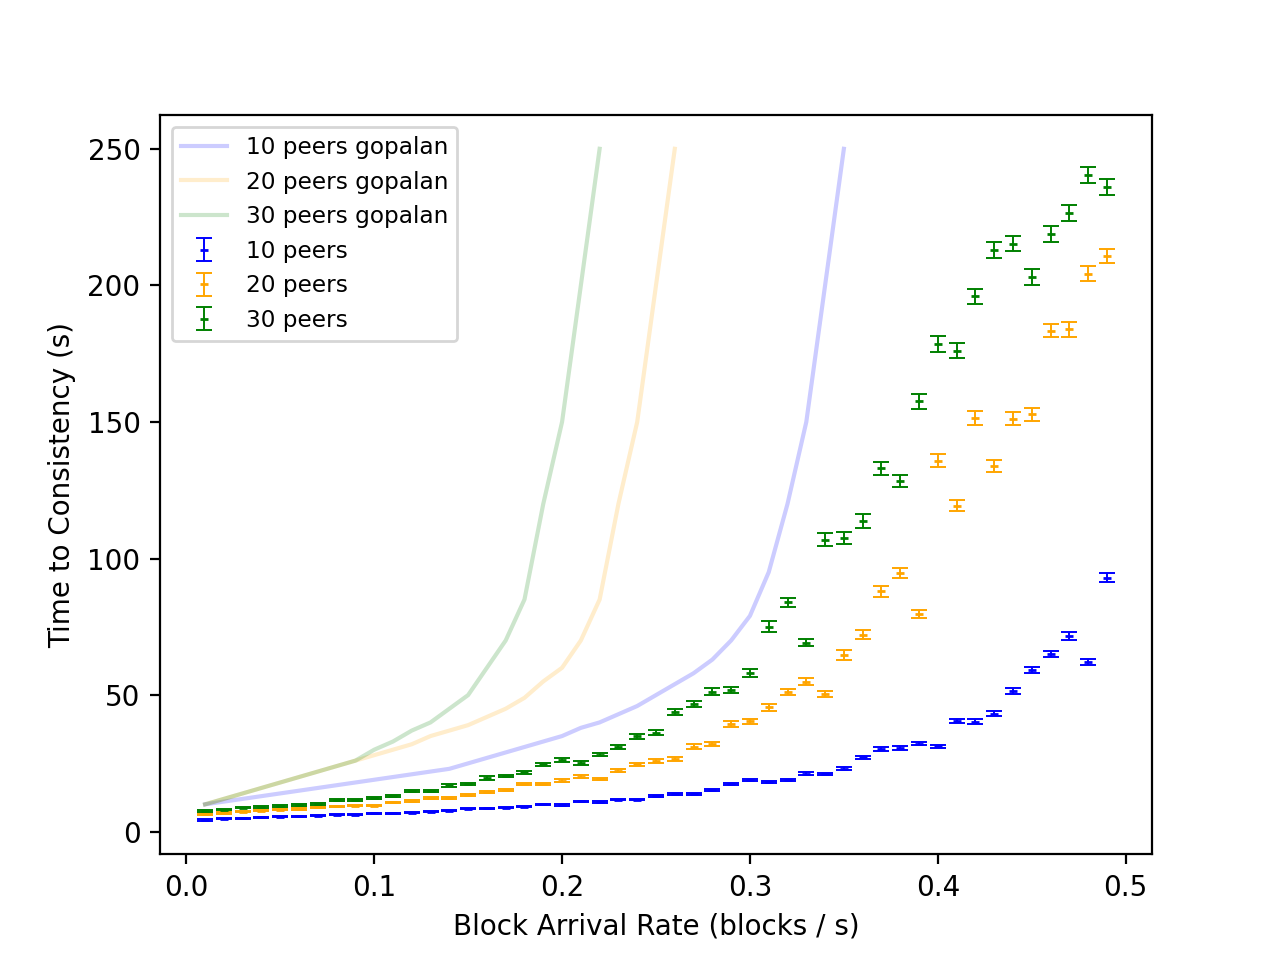
\includegraphics[width=\textwidth]{figures/gopalan_figures/time_to_consistency.png}
		\caption{ Time to Consistency}
		\label{fig:gopalan_ttc}
	\end{subfigure}
	\hfill
	\begin{subfigure}[b]{0.5\textwidth}
		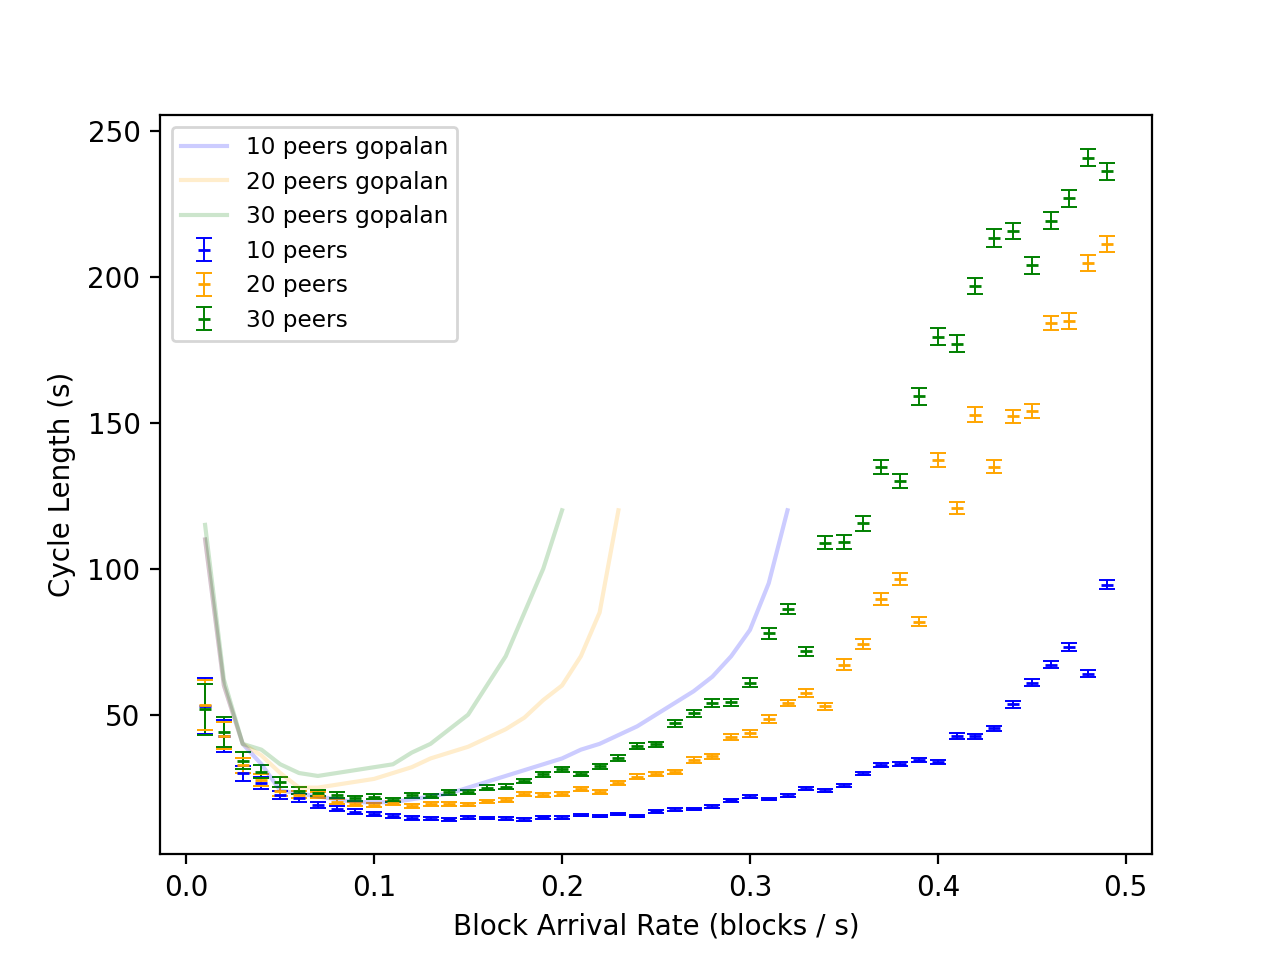
\includegraphics[width=\textwidth]{figures/gopalan_figures/cycle_length_avg.png}
		\caption{ Cycle Length}
		\label{fig:gopalan_cl}
	\end{subfigure}
	\hfill
	\begin{subfigure}[b]{0.5\textwidth}
		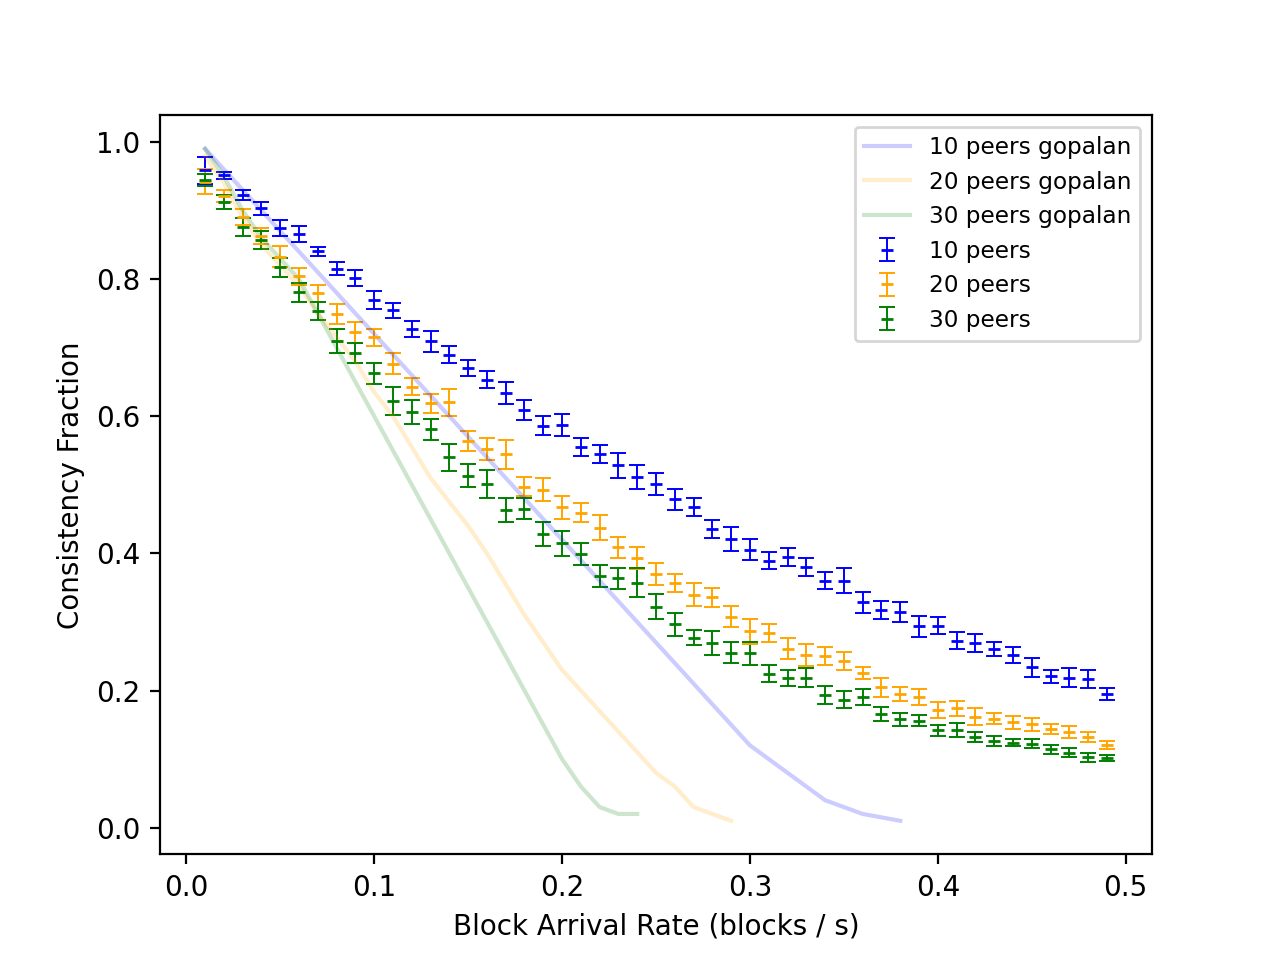
\includegraphics[width=\textwidth]{figures/gopalan_figures/consistency_fraction.png}
		\caption{ Consistency Fraction}
		\label{fig:gopalan_cf}
	\end{subfigure}
	\hfill
	\begin{subfigure}[b]{0.5\textwidth}
		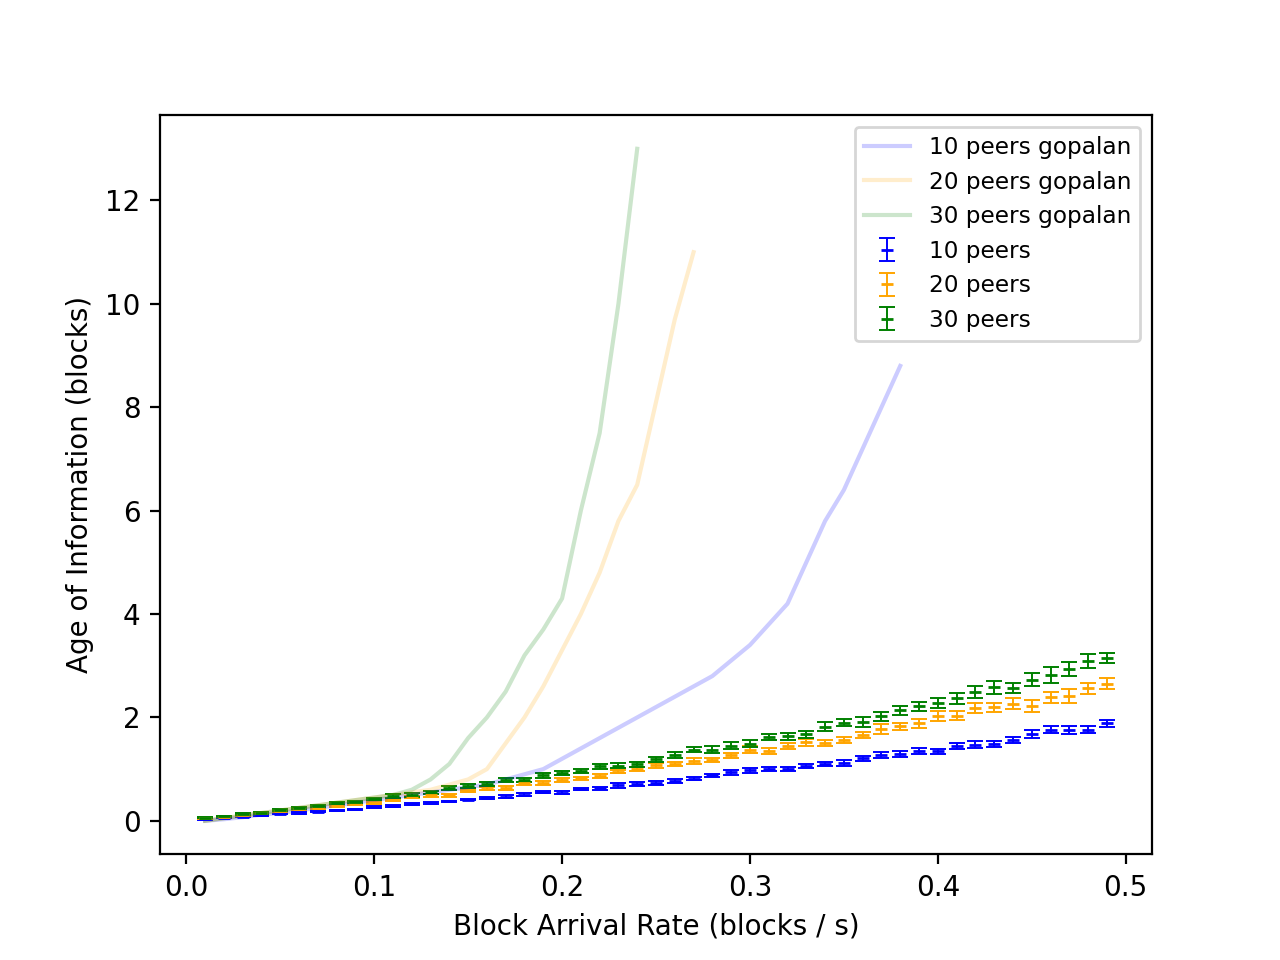
\includegraphics[width=\textwidth]{figures/gopalan_figures/age_of_information.png}
		\caption{ Age of Information}
		\label{fig:gopalan_aof}
	\end{subfigure}
	\caption{Comparison between Simpy Blockchain Simulator and values produced by~\cauth{gopalan}}
\end{figure} 
The metrics of time to consistency and cycle length are very closely related, because both rely on the time the system needs to reach consistency.
Figure~\ref{fig:gopalan_ttc} and Figure~\ref{fig:gopalan_cl} show this close relationship. Additionally the comparison between the Simpy Blockchain Simulator shows a very similar tendency in both metrics. Especially in Figure~\ref{fig:gopalan_ttc} it is observable that the curve has the same shape, only flatter. Figure~\ref{fig:gopalan_ttc} shows that peer number and block arrival rate are proportional to the average time to consistency. Since cycle length is the sum of the average time to consistency and the average of the time the system stays consistent the same behavior can be observed in Figure~\ref{fig:gopalan_cl}. Additionally Figure~\ref{fig:gopalan_cl} shows that for very small numbers for the block arrival rate the cycle length increases again. When the system has a low block arrival rate the system tends to stay longer in a state of consistency, which is due to the fact that the idle time increases.\\
Consistency fraction and age of information are both metrics measuring the consistency of an average peer. The consistency fraction is the fraction of peers, which have a block set equal to $B_G(t)$~\ref{unisondef}. For both the simulation results by~\cauth{gopalan}~and the Simpy Blockchain Simulator we can observe, that the consistency fraction decreases with an increasing blockrate and peer number. While the exact numbers do differ, similar shapes can again be observed.\\
The age of information metric analyzes how much an average peer differs from $B_G(t)$~\ref{unisondef}. It showcases an increase for an increasing blockrate and peer number.
The differences indicate that information spreads faster in the Simpy Blockchain Simulator. After a brief discussion with~\cauth{gopalan}, they confirmed that this might be due to the fact, that in the Simpy version communication processes are handled truly concurrently.	

\subsection{Validation of Simulator against Bitcoin data}
This section validates the model against a real world blockchain system, the Bitcoin network. The Selfish Rumor Model implements an abstract network model of blockchain systems, simulating block creation and block propagation.
\cauth{neudecker-atc16} monitor the Bitcoin network and obtain data of, for example, the current block propagation delay distribution~\cite{BitcoinNetworkMonitor}. Since the model can be used to analyze blocks and their propagation, the current block propagation delay distribution is a suitable metric to compare the Selfish Rumor Model against the real world system.\\
Bitcoin block propagation has two distinct characteristics. The distribution has a high peak at around $~400ms$ and a significant long tail, with block delays going up to $30s$. Since the whole dataset contains many outliers, $5\% $ of the largest delays are filtered out. This data is then used to match parameter setups of the Selfish Rumor Model against Bitcoin and find setups offering a similar block propagation.\\
To achieve a similar block propagation one can mainly analyze the topology of the network graph and the communication process rate.
The current Bitcoin network has an unknown topology. The original protocol described an algorithm, where a peer tries to maintain at least 8 connections~\cite{tschorsch}. This would result in a random regular graph as network topology. However, analysis of the Bitcoin network comes to a different conclusion.\\
For example \cauth{baumann2014exploring} found strong indicators for a scale-free degree distribution.
Additionally, the FIBRE network and Compact Blocks were introduced to enable faster block propagation~\cite{measurement}. This results in a network topology, which cannot be captured by single graph representation.\\
Since the Selfish Rumor Model uses one single graph representation the objective is to utilize a topology and minimize the Root-Mean-Square-Error(RMSE). The RMSE is the standard deviation of the prediction errors~\cite{RMSE}. Since the Selfish Rumor Model Simulator can predict block propagation of Bitcoin, we can measure the error compared to Bitcoins block propagation utilizing the RMSE. Therefore, either a regular random graph or a scale free graph should be chosen as a network topology for the Selfish Rumor Model. 
\begin{figure}[tbp]
	 \begin{subfigure}[b]{0.48\textwidth}
		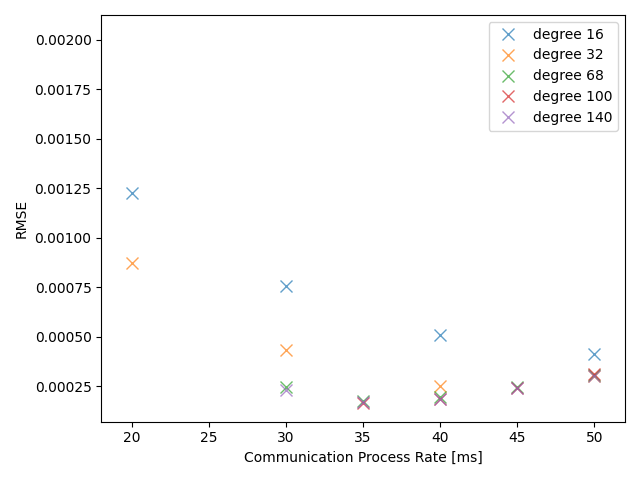
\includegraphics[width=\textwidth]{figures/RMSE_95.png}
		\caption{RMSE between Selfish Rumor Model regular-random Graph and Bitcoin}
		\label{fig:RMSE}
	\end{subfigure}
	\hfill
	\begin{subfigure}[b]{0.48\textwidth}
		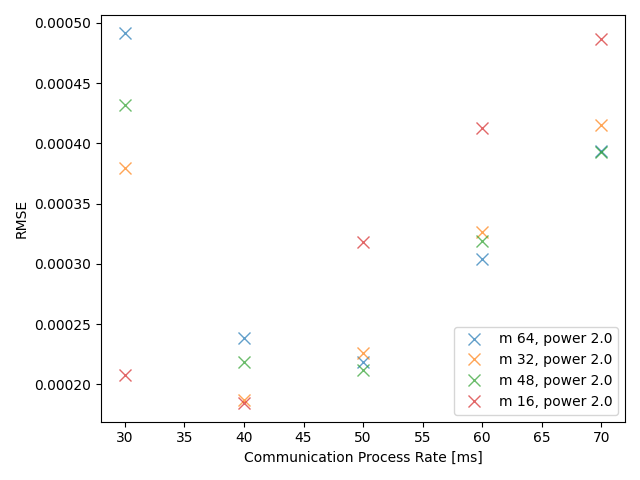
\includegraphics[width=\textwidth]{figures/RMSE_95_barabasi.png}
		\caption{RMSE between Selfish Rumor Model scale-free Graph and Bitcoin}
		\label{fig:RMSEBar}
	\end{subfigure}
	\hfill
	\begin{subfigure}[b]{0.48\textwidth}
		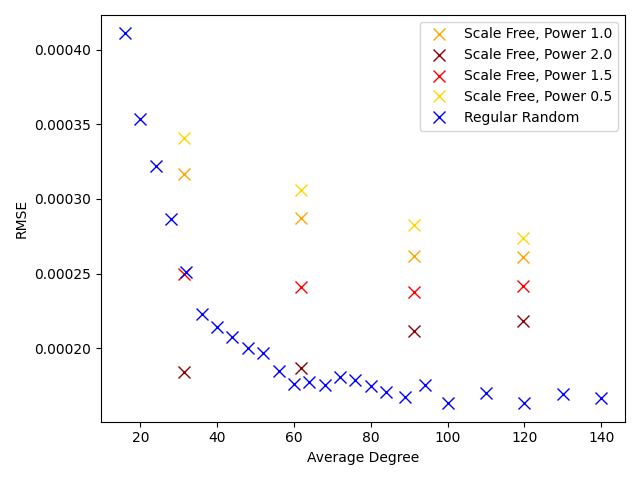
\includegraphics[width=\textwidth]{figures/rmse_min.png}
		\caption{Minimum RMSE value in random-regular graph and scale-free graph}
		\label{fig:minRMSE}
	\end{subfigure}
	\hfill
	\begin{subfigure}[b]{0.48\textwidth}
		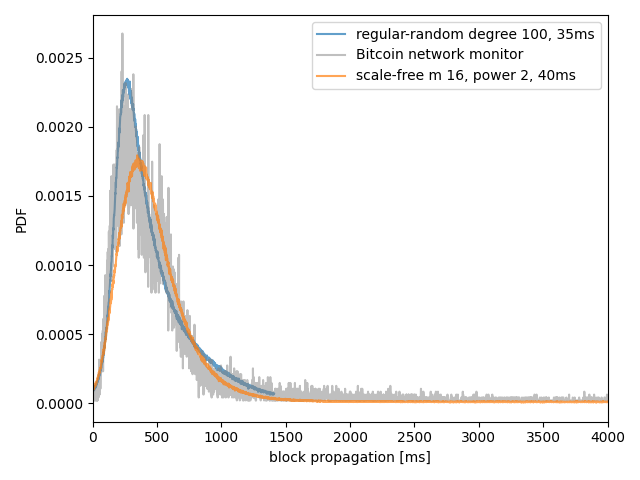
\includegraphics[width=\textwidth]{figures/propagation_histogram_withBitcoin.png}
		\caption{Selfish Rumor Model Model Block Propagation Distribution and Bitcoin}
		\label{fig:SRMBitcoin2}
	\end{subfigure}
\caption{Selfish Rumor Model Experiments in comparison with Bitcoin, 500 Peers}
\label{fig:SMRBitcoin}
\end{figure}
Figure~\ref{fig:SMRBitcoin} shows the most important results of various experiments carried out to minimize the RMSE between the simulations and Bitcoin. It also offers a comparison between the scale-free topology shown as orange and the regular random topology shown as blue. Since both topologies differ only in the degree distribution, we can compare both by their average degree respectively. All block delays were grouped in $1ms$ steps. All setups were repeated 100 times to ensure statistical significance.\\
Figure~\ref{fig:RMSE} shows the RMSE for 16, 32, 68, 100, 140 degrees and various communication process rates in comparison to Bitcoin. The lowest RMSE, $0.00016$, was achieved by 100-regular-random graph with a communication process rate of $35ms$. This parameter setup is referred to as $RegRan$.\\
In Addition the results for a 16- and 32-regular-random graph are also shown in Figure~\ref{fig:RMSE}. A 32 degree regular random graph is used by~\cauth{gopalan}~to evaluate against Bitcoin data. However, the RMSE-values are significantly higher than those of the 100-regular-random graph. This is most likely due to the usage of the FIBRE relay network and Compact Blocks in Bitcoin, which decreases block propagation delay. Additionally, all curves have a clear tendency towards a specific communication rate minimizing the RMSE.\\
This is also the case for scale-free networks, as is visualized in Figure~\ref{fig:RMSEBar}. For each topology there is one minimum communication rate, minimizing the RMSE against Bitcoin block propagation delay distribution. The scale-free network is generated over the Barabasi-Albert model~\cite{BarabasiAlbert}. This algorithm has three determining parameters. The number of vertices, $m$ for the number of edges generated for each vertex and a power factor. Since the lowest RMSE was always achieved for the power factor $2$ Figure~\ref{fig:RMSEBar} shows only the RMSE for power $2$.\\
The lowest achieved RMSE, $0.00018$, for scale free networks was for an average of 16 m, a power factor of 2 and a communication process rate of 40ms. This parameter setup is referred to as $ScaFre$.\\
Both topologies achieve quite low RMSE values. However, Figure~\ref{fig:minRMSE} visualizes the difference between the minimum RMSE values achieved for each average degree for both random regular and scale free graphs.
Regular random graphs lower the RMSE values for an increasing average degree, until an average degree of 80. Above an average degree of 80 the RMSE values remain quite constant.\\
The analysis of parameter setups for scale free networks is more complex. Scale-free networks, in terms of the Barabasi-Albert model, have the parameter m, which can be used to control the average degree of the network. Additionally scale-free networks have a power factor, which controls the preferential attachment process. Since 4 different power factors were analyzed for each setup, Figure~\ref{fig:minRMSE} visualizes 4 data points above each other for each average degree. We can observe that for $m=16$ and for $m=32$ the achieved RMSE values are the lowest for power factor 2 and a communication process rate of 40ms.\\
Figure~\ref{fig:SRMBitcoin2} visualizes the block propagation distribution from the Selfish Rumor Model for both tested topologies in their minimum configuration and Bitcoin. The regular random graph models the peak closer. The scale free network cannot model the peak as good as the regular random network, but the curve shows more distinctly the long-tail behavior. The better model for lower delays achieves a better RMSE value, since lower delays contain much more data points. Since data points above 1500ms are rare for Bitcoin, the exact modeling of the long tail does not impact the RMSE value as much. Nonetheless, both parameter setups are valuable to establish a validated Selfish Rumor Model Setup.\\
We conclude this section by establishing two parameter setups. The minimum configuration for regular random networks is called $RegRan$ and the minimum configuration for scale-free networks is called $ScaFre$. Both are discussed in their differences in the above chapter exhaustively. However, there are also characteristics both share.\\
The interarrival time of the block arrival process is set to 600s. In a scenario, where multiple blocks could be transferred from one peer to another the block with the earliest arrival time is chosen. The number of peers is set to 500 and the mining power distribution is exponential. Additionally Simulations are always carried out 100 times to ensure statistical significance.
Those parameter setups, $RegRan$ and $ScaFre$ are used for following evaluations.

\section{Selfish Mining and Networking Effects}
Networking effects and selfish mining can be analyzed from a global and a local point of view, cf. Table~\ref{keyfactors}. The system analysis introduced by~\cauth{gopalan}~assesses the system mainly in terms of consistency and blockchain growth, as discussed in the previous section. Both, blockchain growth and consistency, are influenced by adversarial mining strategies such as selfish mining. Additionally, selfish mining is influenced by networking factors.

\subsection{Selfish Mining in homogeneous Network Setting}
\citeauthor{eyal}~\cite{eyal} discovered a relationship between the relative computational power and the resulting $revenue~gain$. They described that an increase in networking propagation factor and relative computational power results in an increased $revenue~gain$. Additionally to the metrics of $revenue~gain$ and network propagation factor $\gamma_{hr}$ we introduce two other metrics. Those are $growth$ and $fork~rate$. $growth$ describes the length of the blockchain relative to the number of produced blocks and $fork~rate$ describes the number of forks relative to the number of blocks~\cite{BlockPropOld}. A high $growth$ means that most produced blocks end up in the longest chain. If the $fork~rate$ is significantly smaller than $1-growth$ this implies that forks tend to contain many blocks. If it is close to equal forks are mostly consisting of one block.\\
In a homogeneous network every peer has the same degree and the same bandwidth. Such a network setup is the $RegRan$ setup and it can be used to analyze selfish mining in a scenario without any networking advantage.
\begin{figure}[tbp]
	 \begin{subfigure}[b]{0.5\textwidth}
		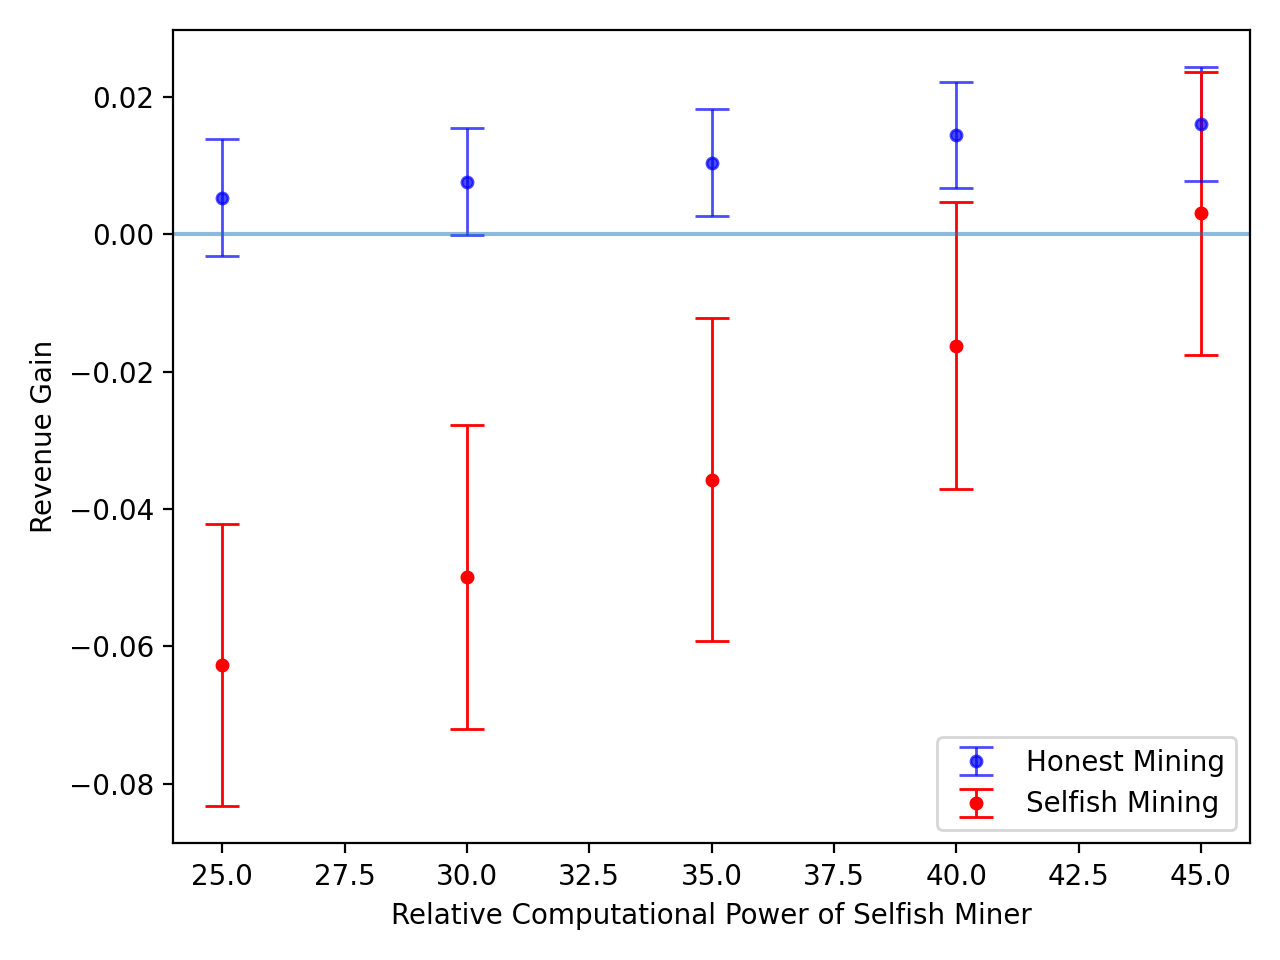
\includegraphics[width=\textwidth]{figures/rev_and_bpr_per_peer.png}
		\caption{Revenue Gain\\ with Standard Deviation}
		\label{fig:multi_hr}
	\end{subfigure}
	\hfill
	\begin{subfigure}[b]{0.5\textwidth}
		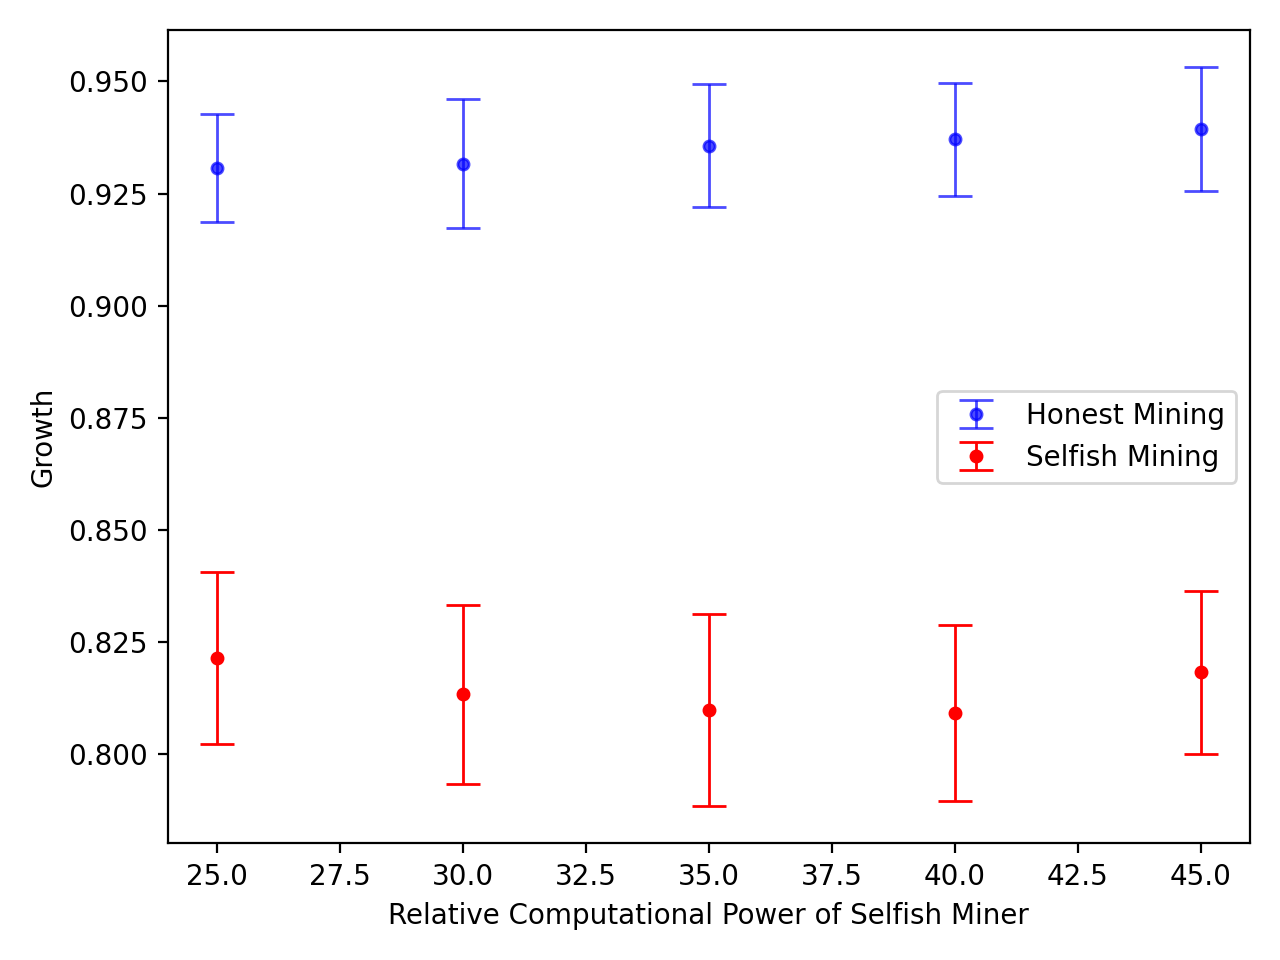
\includegraphics[width=\textwidth]{figures/growth.png}
		\caption{Relative Average Growth of Blockchain \\with Standard Deviation}
		\label{fig:multi_hr_growth}
	\end{subfigure}
	\caption{Simulations $RegRan$ Setup, multiple Hashrates, Comparison between peer with ID $0$ executing honest and selfish mining}
	\label{fig:mhr}
\end{figure}
Figure~\ref{fig:multi_hr} shows the $revenue~gain$ for relative computational power between $25\% $ and $45\% $. Figure~\ref{fig:multi_hr} shows that for selfish mining the $revenue~gain$ is on average below zero except for $45\% $ relative computational power. For honest mining it is above zero. This shows that in this scenario honest mining is outperforming selfish mining. Increasing the relative computational power also increases $revenue~gain$ for the selfish miner. The small $revenue~gain$ of the honest miner increases as well, but only very slightly. The $revenue~gain$ has a greater standard deviation for the selfish miner than for the honest miner. Especially for the selfish miner $revenue~gain$ is wide spread. Nonetheless, the results contradict the \cauth{eyal} since the authors showed a strict revenue increase for $\alpha > 33\% $. Since $\alpha$ can be seen as the fraction of blocks a miner produces it is directly linked to the relative computational power this miner possesses. Thus, according to \cauth{eyal} Figure~\ref{fig:multi_hr} should be positive for the relative computational power greater than $33\% $, which is very clearly not the case.\\
The overall $growth$ of the blockchain is influenced by the selfish mining protocol, as is visualized in \ref{fig:multi_hr_growth}. $growth$ is the length of longest chain divided by the number of produced blocks. In an ideal case the $growth$ of the blockchain is $1$ for a complete honest network. However, network effects result in a $growth$ $~93\% $ even in a total honest network. This also explains the $revenue~gain$ of the honest miner. Since the blockchain contains forks, a peer producing a large amount of blocks will gain more revenue than its relative share. We can observe as well that selfish mining lowers the overall $growth$ of the blockchain, as expected. For the setup containing the selfish miner the overall $growth$ remains constant at around $82\% $. Note, that the $growth$ reduction seems to be independent of the relative share of computational power the selfish miner possesses, at least for relative computational powers between $25-45\% $.
Selfish mining in an homogeneous network setting does not result in a $revenue~gain$ compared to honest mining.

\subsection{Selfish Mining with Network Advantage}
Selfish Mining in a homogeneous network is not beneficial. Therefore, analysis is conducted in network settings, where the selfish miner possesses a network advantage. In the following evaluations peer with ID $0$ will possess a network advantage. This peer executes selfish and honest mining. This allows us to compare the impacts of networking advantage on honest and selfish mining. In the following experiments the selfish miner possesses a relative computational power of $45\% $.

\paragraph{Selfish Mining with Network Advantage in \textit{RegRan}}
The $RegRan$ setup utilizes a regular random graph as network topology. Increasing degree and accelerating communication process rate results in a networking advantage.
\begin{figure}[tbp]
	 \begin{subfigure}[b]{\textwidth}
		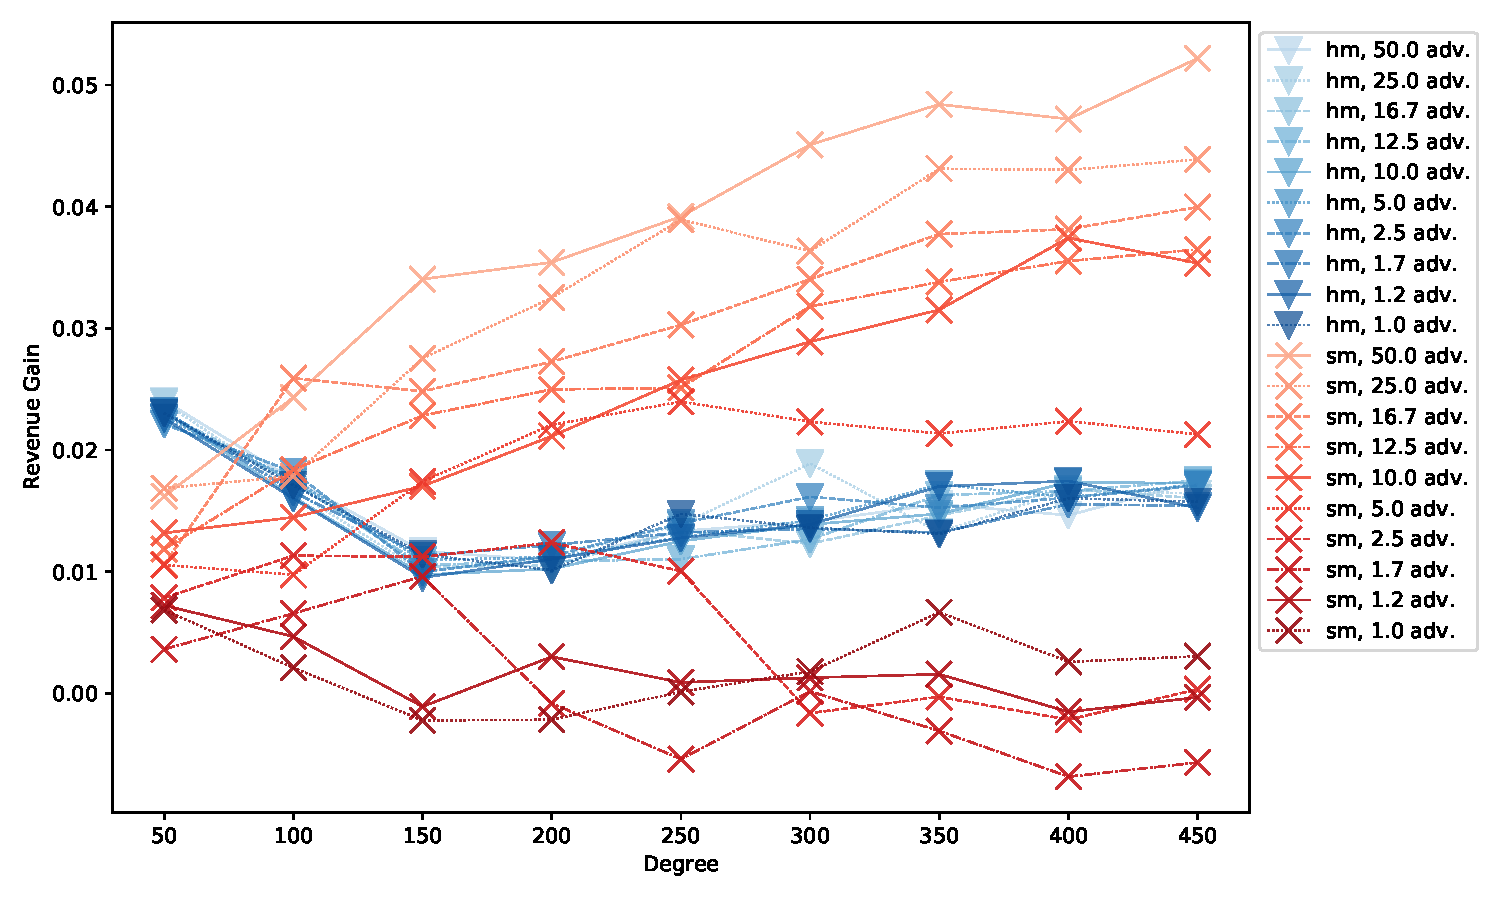
\includegraphics[width=\textwidth]{figures/sm_edge_new_revenue.pdf}
		\caption{Revenue Gain}
		\label{fig:sm_edge_rev}
	\end{subfigure}
	\hfill
	\begin{subfigure}[b]{\textwidth}
		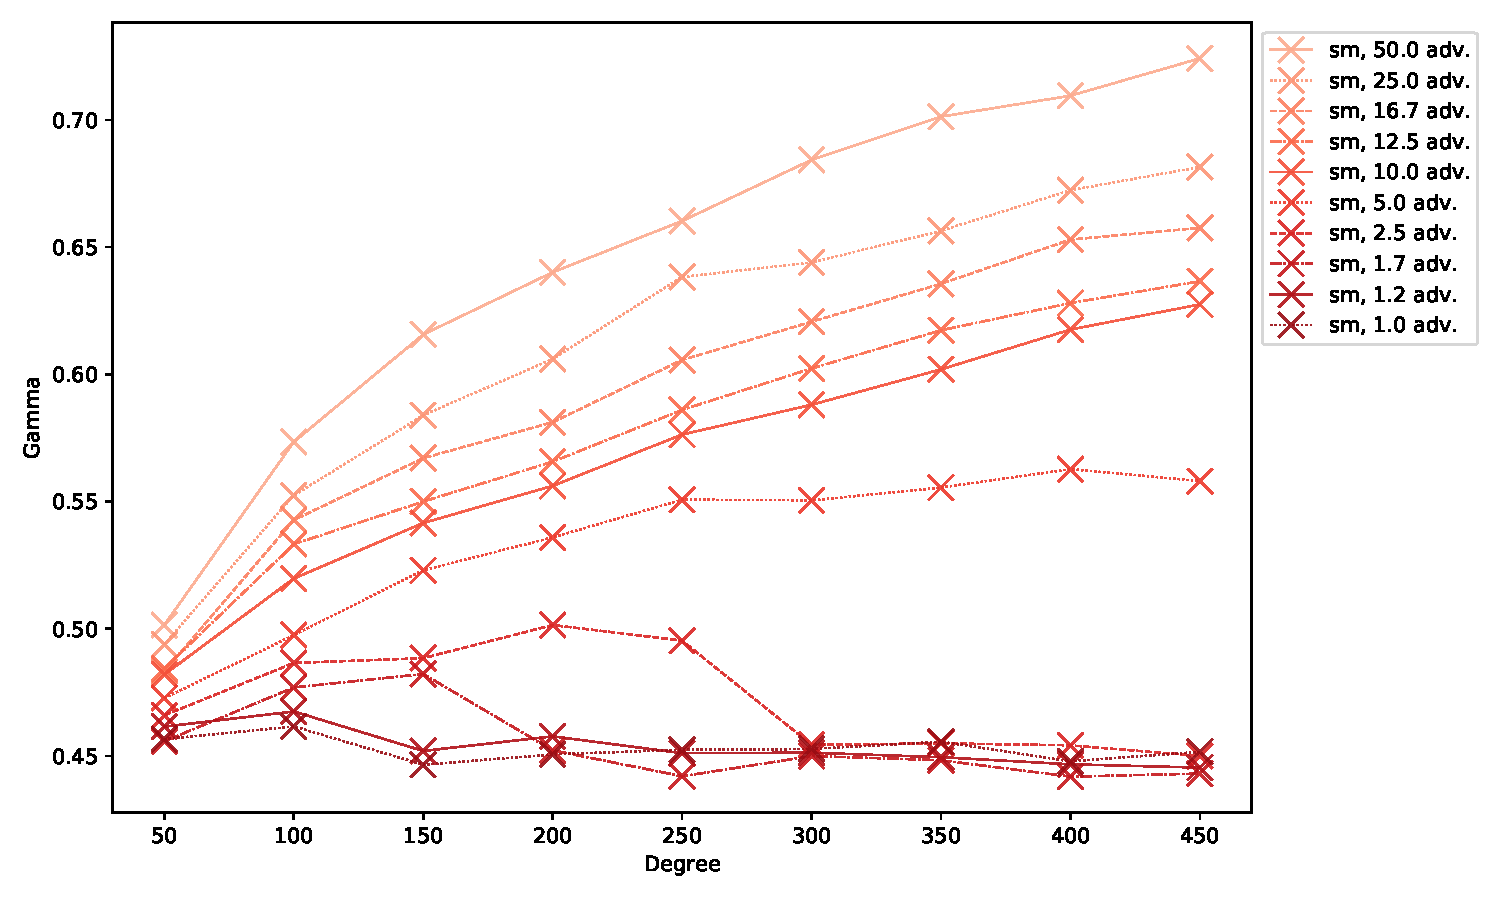
\includegraphics[width=\textwidth]{figures/sm_edge_new_gamma.pdf}
		\caption{Network Propagation Factor $\gamma_{hr}$}
		\label{fig:sm_edge_gamma}
	\end{subfigure}
		\caption{Simulations $RegRan$ Setup with Network Advantage for honest mining(hm) and selfish mining(sm), Different Communication Process Rates Advantages, $revenue~gain$ and $\gamma_{HR}$}

\end{figure}
\begin{figure}[tbp]
\begin{subfigure}[b]{\textwidth}
		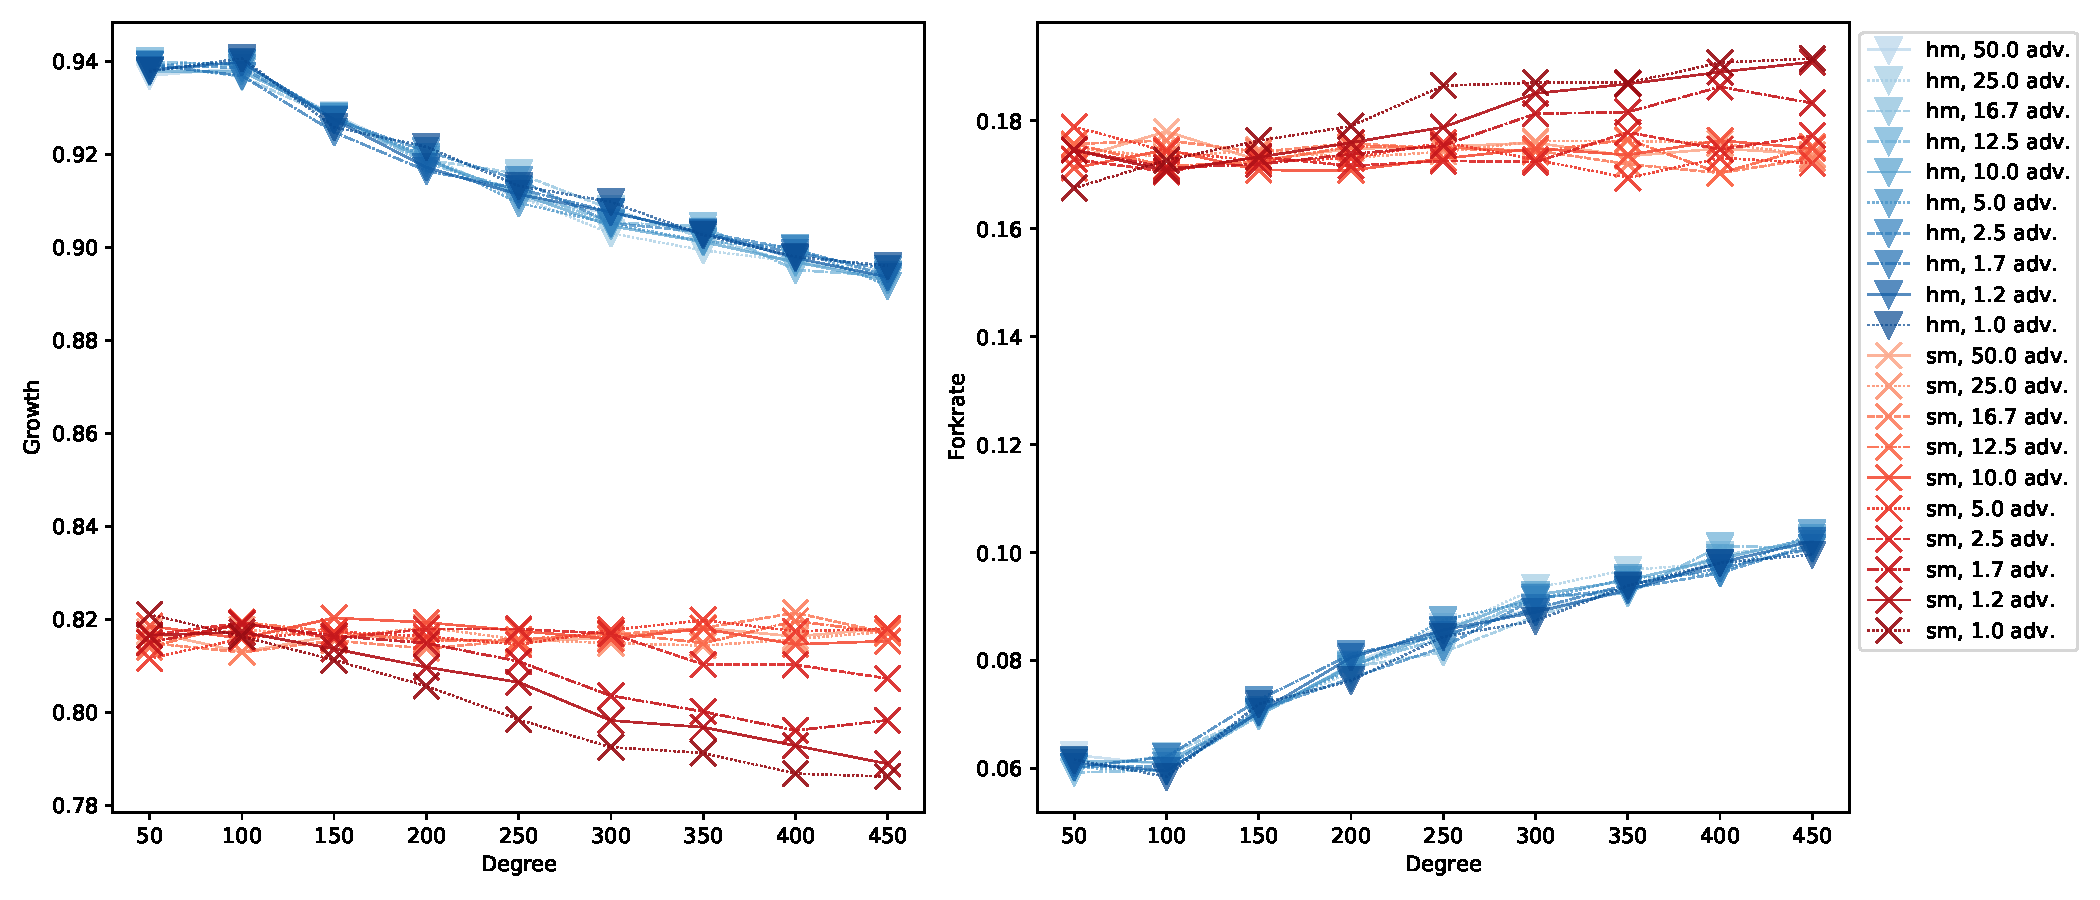
\includegraphics[width=\textwidth]{figures/sm_edge_new_growth_and_forkrate.pdf}
		\caption{Growth and Fork~rate}
		\label{fig:growth_fork}
	\end{subfigure}
\caption{Simulations $RegRan$ Setup with Network Advantage for honest mining(hm) and selfish mining(sm), Different Communication Process Rates Advantages, $growth$ and $fork~rate$}
\label{fig:sm_edge_new}
\end{figure}
Figure~\ref{fig:sm_edge_new} visualizes experiments with network advantage. We consider peer with ID $0$ executing both mining strategies and alter his network parameters. The main metric to analyze mining protocols is $revenue~gain$, which is visualized in \ref{fig:sm_edge_rev}. We can observe that selfish mining results in a more spread out $revenue~gain$ than honest mining. Additionally to an increased degree the communication process rate was increased by an advantage factor, which is shown in the legend. We can observe that for almost all cases a higher advantage factor results in more $revenue~gain$. We can also observe that increasing degree does not necessarily result in an increased $revenue~gain$, in fact it may even result in a revenue loss. This is an intuitive result since in a real system splitting bandwidth between an increasing number of connections may at one point result in an overall worse performance. However, increasing both advantage factor and degree results in an overall increased $revenue~gain$.\\
Figure~\ref{fig:sm_edge_gamma} visualizes the network propagation factor $\gamma_{hr}$. It is a metric only applicable to selfish mining, since it analyzes contest situations. It shows the fraction of the network receiving the selfish miner block before the contestant block. If we compare Figure~\ref{fig:sm_edge_gamma} and \ref{fig:sm_edge_rev} we observe a clear correlation between an increasing $\gamma_{hr}$ and $revenue~gain$. The curve for the $5$-times advantage factor even visualizes that if $\gamma_{hr}$ stagnates, the $revenue~gain$ does so as well. The $2.5$-times advantage factor curve shows at $300$ degree, that if $\gamma_{hr}$ drops significantly below $50\% $, the selfish mining $revenue~gain$ drops below the honest mining $revenue~gain$.\\
Honest mining is mostly unaffected by changes in advantage factor, but very much affected by changes to the degree of the miner. However, in comparison to the $revenue~gain$ of the selfish miner the honest miner $revenue~gain$ is quite constant. The honest miner shows the highest $revenue~gain$ for a degree less than the network average. This $revenue~gain$ quickly decreases until $150$ were it starts increasing again. If we observe $growth$ and $fork~rate$ in Figure~\ref{fig:growth_fork} we can see that for the degree $50$ and $100$ the $growth$ of the blockchain is the highest and constant for the honest miner scenarios. For degrees larger than $100$ the $growth$ starts rapidly decreasing. We observe the inverse behavior for the $fork~rate$. Since the $fork~rate$ is close to $1-growth$ the forks are very small and we can not observe a network consensus partition. For a degree greater than $150$ we can find a relationship between increasing $revenue~gain$ due to decreasing $growth$. Since the relative computational power of the miner is $45\% $ he profits from a decreased $growth$. However, the increased $revenue~gain$ for degree $50$ and $100$ with a relatively high $growth$ of $94\% $ implies that there exists a $growth$ threshold were the honest miner benefits from a better growth. We presume, that relatively more of his blocks are included in the blockchain if the growth surpasses a certain threshold.\\
The selfish miner scenarios show mostly a very similar low $growth$ and high $fork~rate$. For lower advantage factors $growth$ decreases correlate to a decreased $revenue~gain$. This is most likely due to the fact, that the selfish miner can not effectively push his blocks in the main chain of the blockchain, resulting in a decreased $growth$ and increased $fork~rate$. However, independent of mining strategy we observe $fork~rate \approx 1-growth$ which implies that for both mining strategies we only observe small forks.

\paragraph{Selfish Mining with Network Advantage in \textit{ScaFre}}
The $ScaFre$ setup utilizes a scale free graph as network topology, implying that node degrees are exponentially distributed. To achieve a network advantage for peer with ID $0$, we removed the edges, that were constructed through the Barabasi-Albert Algorithm and then connected peer with ID $0$ to a new amount of peers. The strategies to connect peer with ID $0$ are uniformly at random and according to betweenness centrality. Betweenness centrality is a measure to express how central a node is in a given graph. It is the number of shortest paths that pass through the node\cite{bcent}.
\begin{figure}[tbp]
	 \begin{subfigure}[b]{\textwidth}
		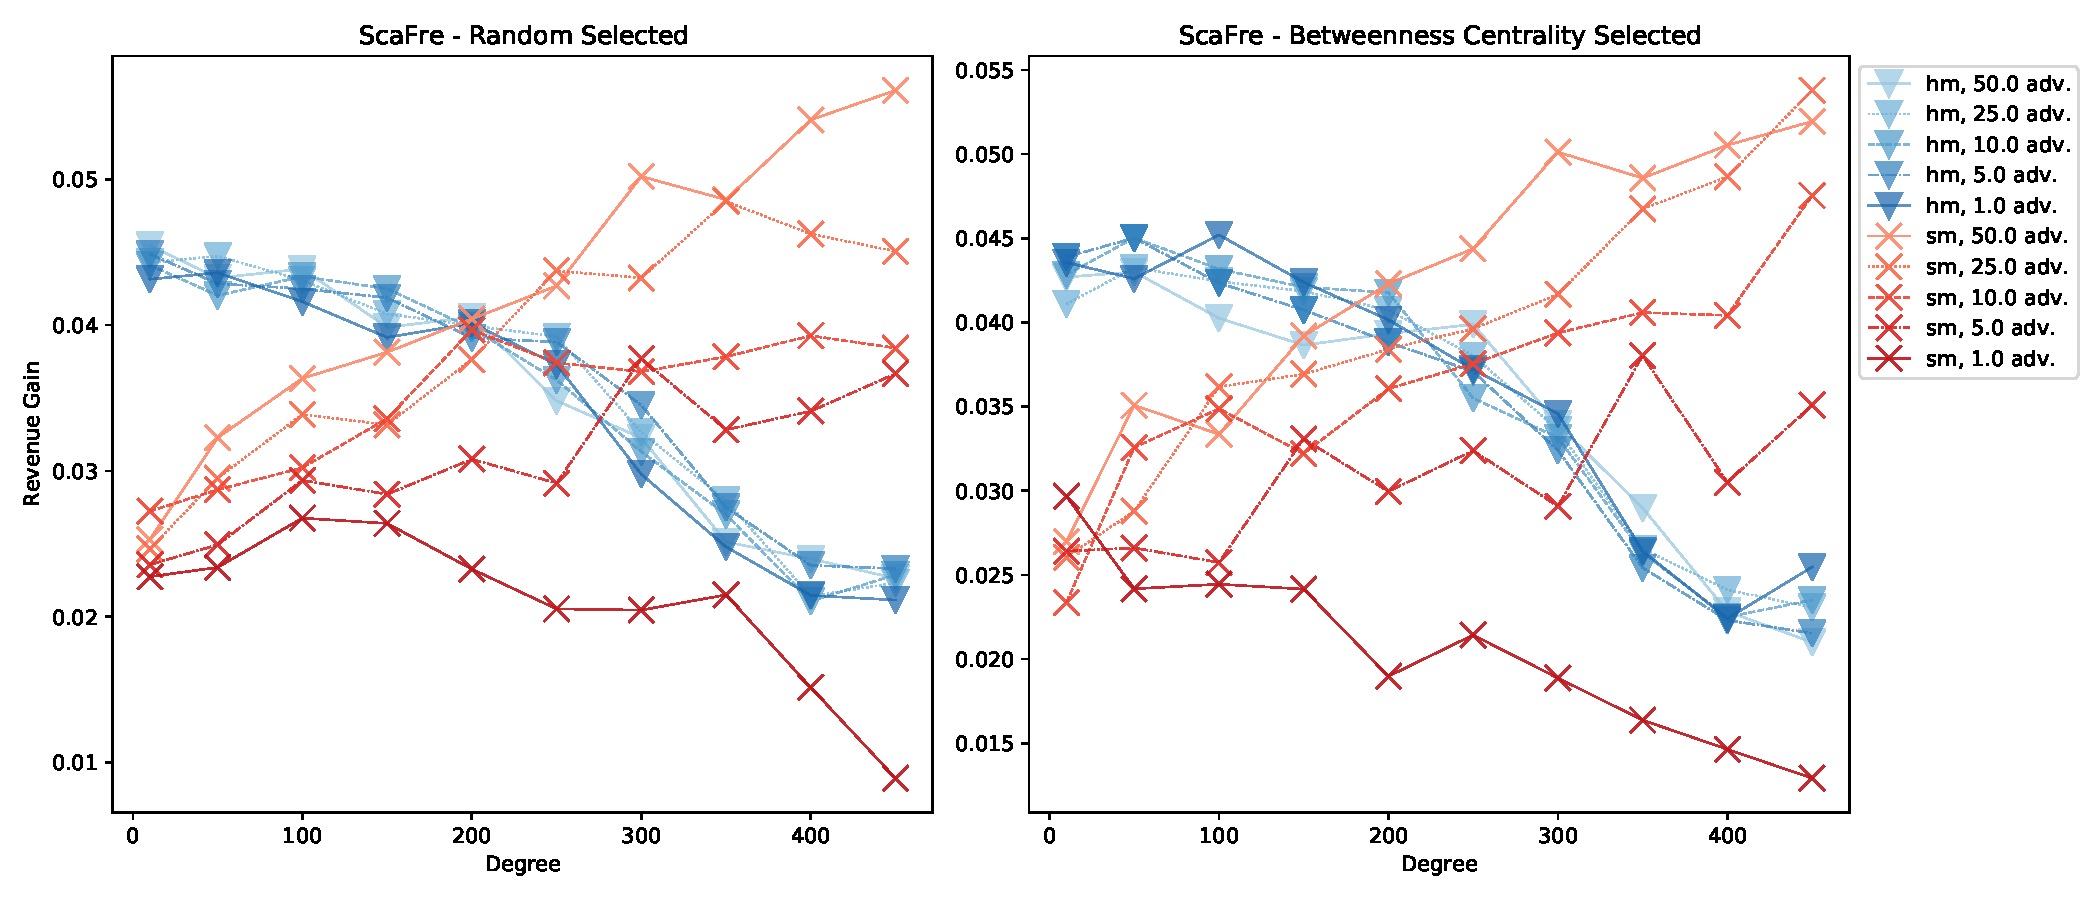
\includegraphics[width=\textwidth]{figures/sm_edge_revenue_barabasi.pdf}
		\caption{Revenue Gain}
		\label{fig:sm_edge_rev_bara}
	\end{subfigure}
	\begin{subfigure}[b]{\textwidth}
		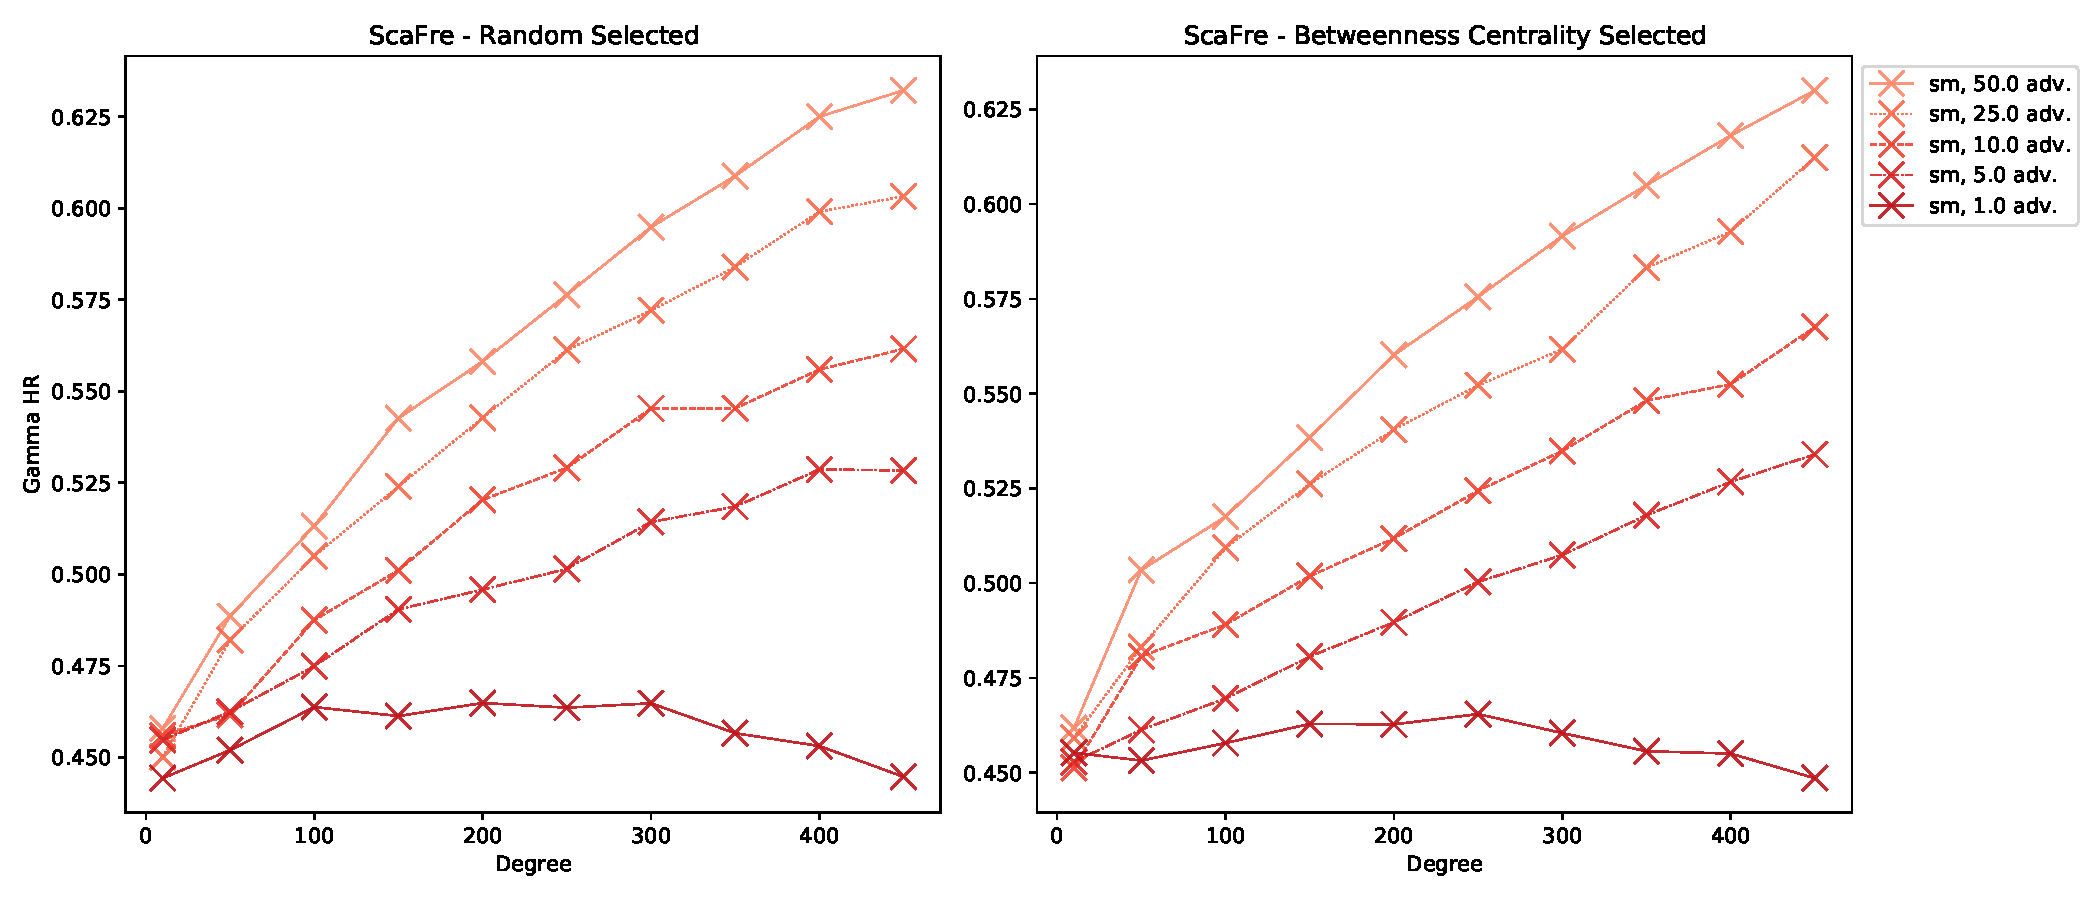
\includegraphics[width=\textwidth]{figures/sm_edge_gamma_barabasi.pdf}
		\caption{Network Propagation Factor $\gamma_{hr}$}
		\label{fig:sm_edge_gamma_bara}
	\end{subfigure}
	
	\caption{Simulations $ScaFre$ Setup with Network Advantage for honest mining(hm) and selfish mining(sm), Different Communication Process Rates Advantages, $revenue~gain$ and $\gamma_{HR}$}
\end{figure}
\begin{figure}[tbp]
\begin{subfigure}[b]{\textwidth}
		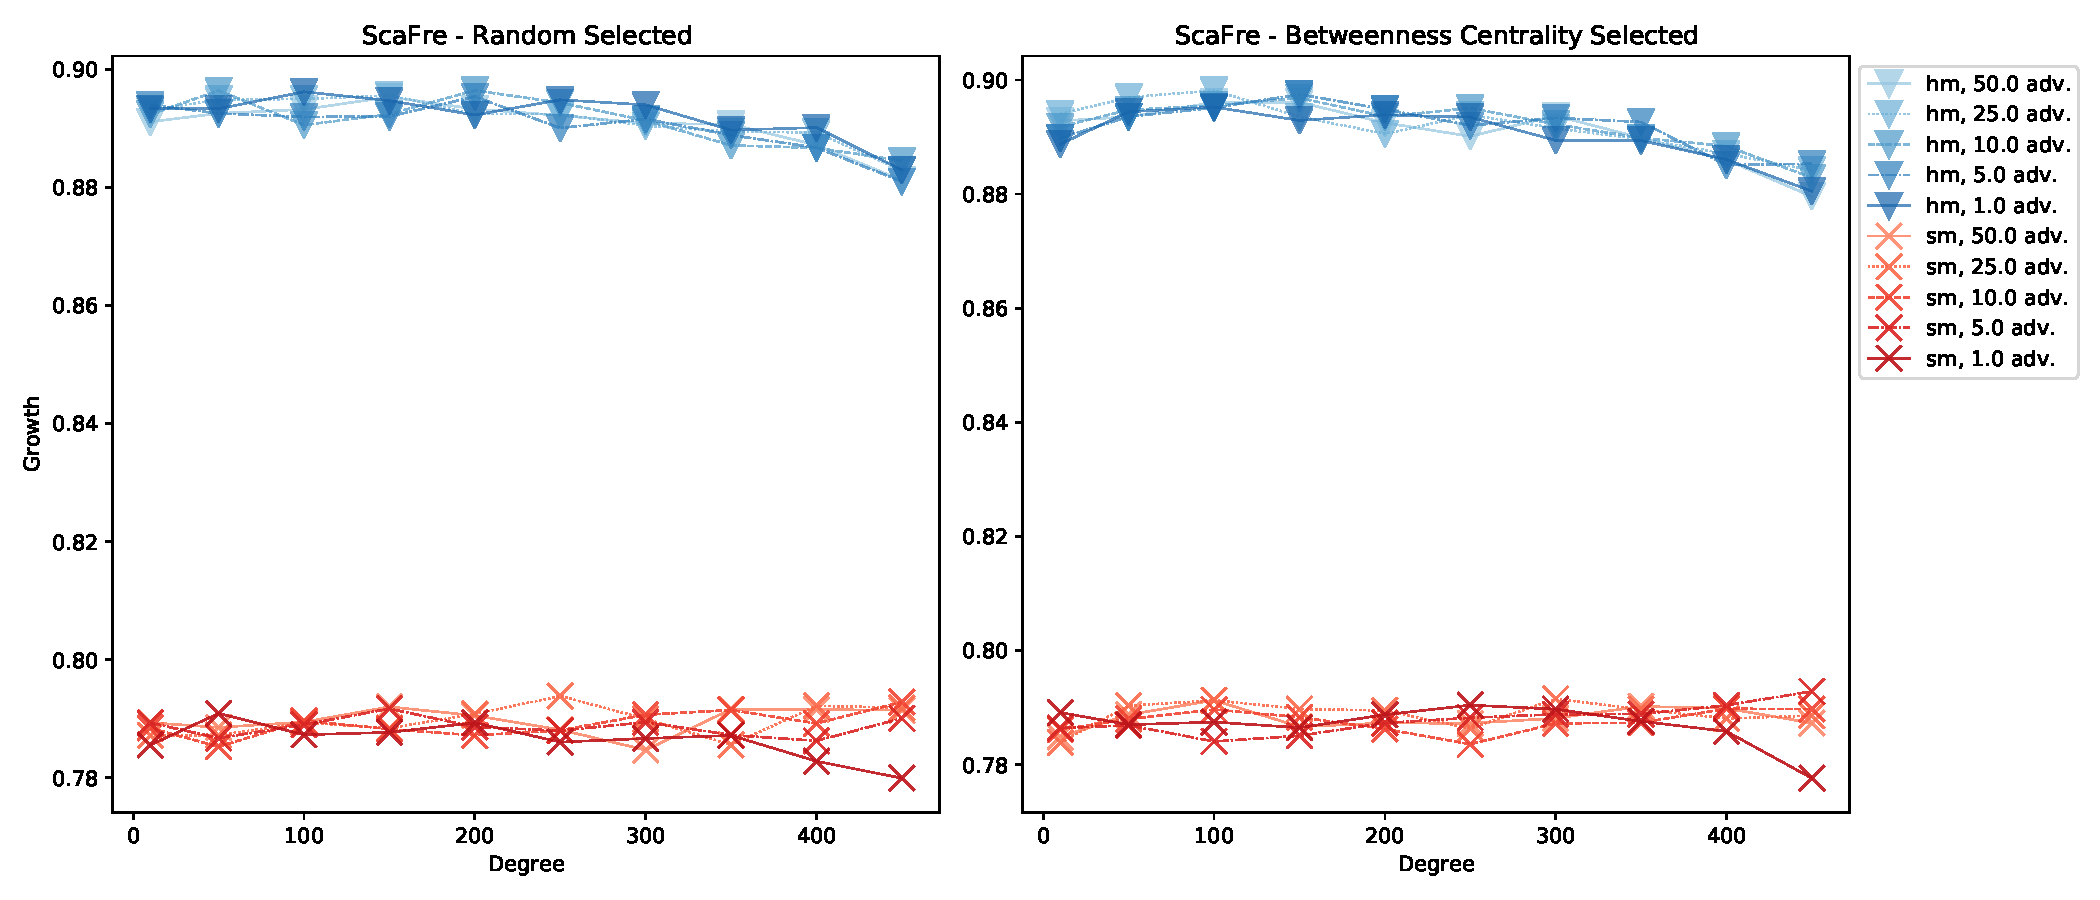
\includegraphics[width=\textwidth]{figures/sm_edge_growth_barabasi.pdf}
		\caption{Growth}
		\label{fig:growth_bara}
	\end{subfigure}
	\begin{subfigure}[b]{\textwidth}
		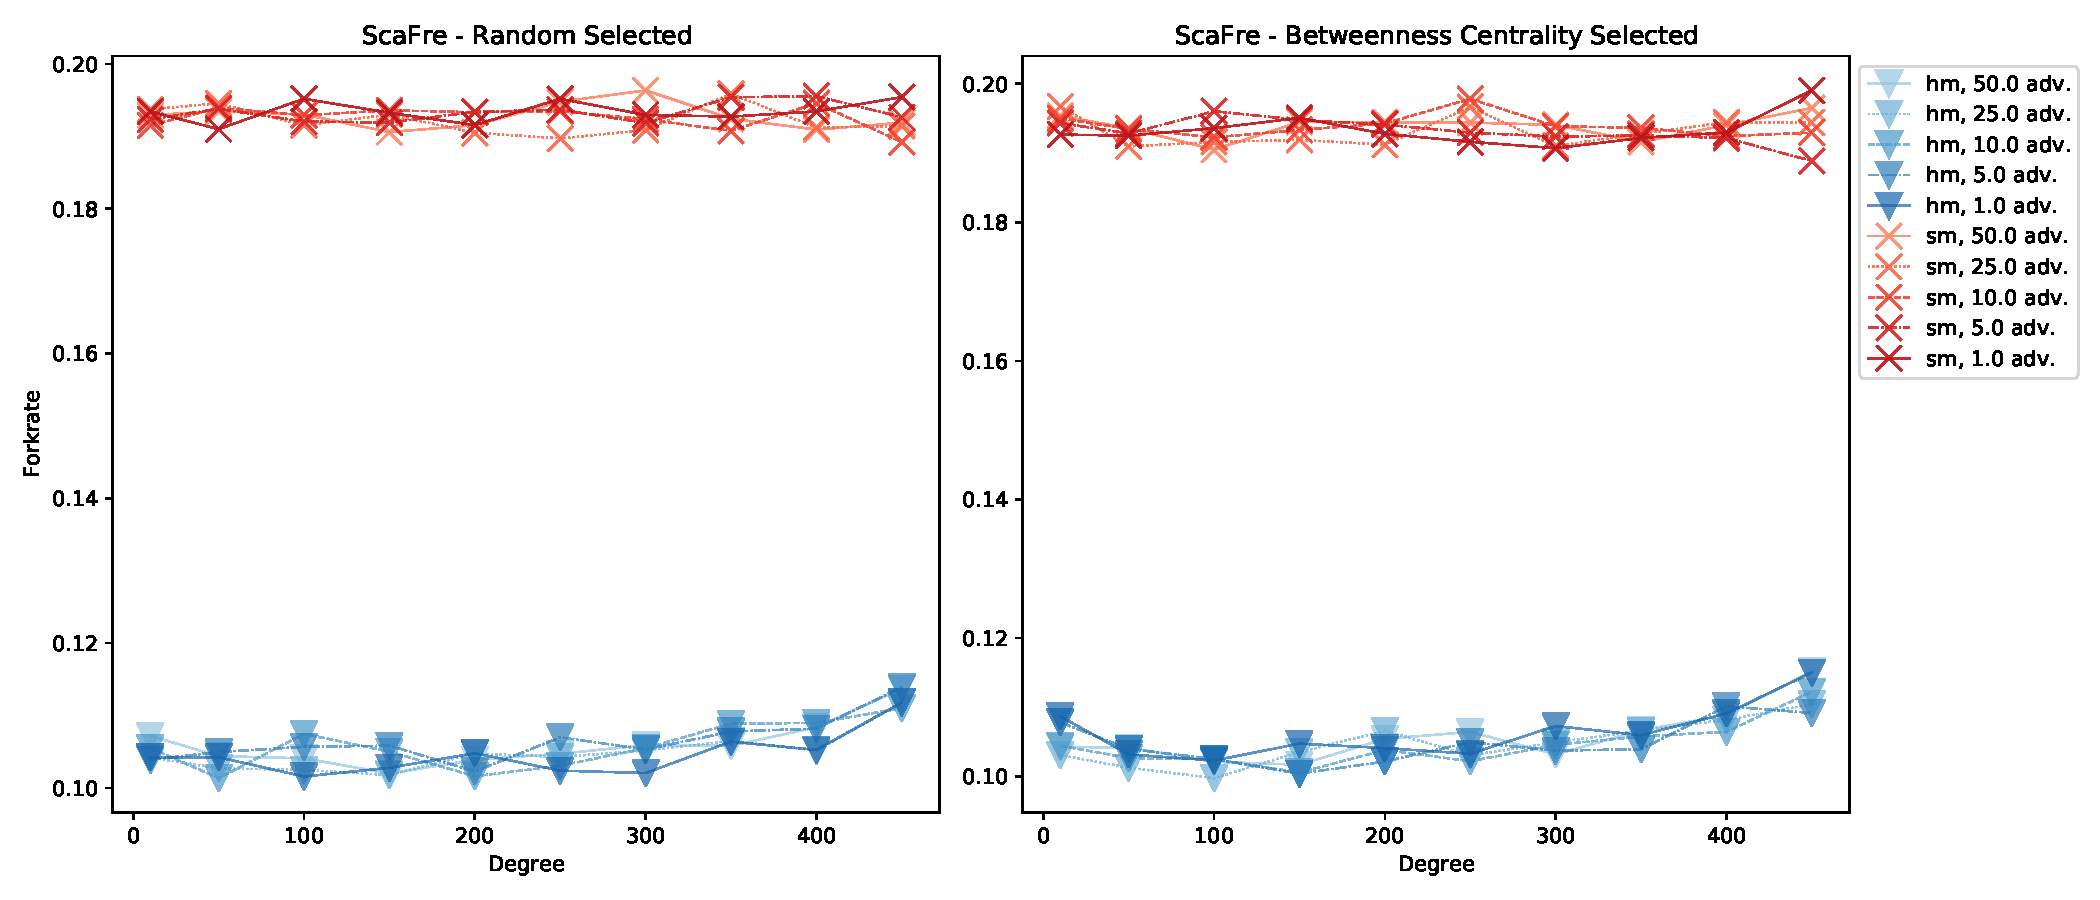
\includegraphics[width=\textwidth]{figures/sm_edge_forkrate_barabasi.pdf}
		\caption{Fork Rate}
		\label{fig:fork_bara}
	\end{subfigure}
\caption{Simulations $ScaFre$ Setup with Network Advantage for honest mining(hm) and selfish mining(sm), Different Communication Process Rates Advantages, $growth$ and $fork~rate$}
\label{fig:sm_edge_barabasi}
\end{figure}\\
Figure~\ref{fig:sm_edge_barabasi} visualizes the results of network advantage simulations carried out in the $ScaFre$ parameter setup. Overall we cannot observe a major difference between the measured metrics in Figure~\ref{fig:sm_edge_barabasi} between both peer selection strategies. Figure~\ref{fig:sm_edge_rev_bara} shows the $revenue~gain$ for honest mining and selfish mining for both strategies. For selfish mining we see a similar dependence of $revenue~gain$ to increasing degree and communication process rate advantage as in the $RegRan$ setup. Selfish mining results in a more spread out $revenue~gain$ than honest mining. An increase in both degree and communication process rate results in a higher revenue gain. If degree and communication process rate surpass a certain threshold, selfish mining produces more revenue gain than honest mining. This threshold is at least a 30-times faster communication process rate and a degree of 250 or higher for both strategies.\\
We also see the same clear correlation between an increasing $\gamma_{hr}$ and $revenue~gain$. A $\gamma_{hr}$ significantly higher than $50\% $ results in a significant $revenue~gain$ for the selfish miner. As expected the highest $\gamma_{hr}$ results in the highest $revenue~gain$ for the selfish miner.\\
A major difference to the $RegRan$ setup is the $revenue~gain$ of the honest miner in the $ScaFre$ setup. The honest miner has a very high $revenue~gain$ with low degrees, which decreases as degree increases. This is in contrast to the $RegRan$ experiments where  $revenue~gain$ remained quite constant with changing degrees for the honest miner. However, in both setups $revenue~gain$ for the honest miner is independent of communication process rate advantage. We observe the highest $revenue~gain$ of $~0.045$ to be at 10-degrees for the honest miner.\\
Figure\ref{fig:growth_bara} and Figure\ref{fig:fork_bara} visualize both $growth$ and $fork~rate$. Both metrics are quite constant for both peer selection strategies and as expected selfish mining leads to a lower $growth$ and higher $fork~rate$. Additionally changes in degree as well as communication process rate advantage do not change $growth$ or $fork~rate$ significantly. This is true for both peer selection strategies and for selfish mining as well as honest mining. Compared to $RegRan$, $ScaFre$ experiments seem to have an overall lower $growth$ and higher $fork~rate$. The relationship of $fork~rate \approx 1-growth$ remains. Communication process rate advantage changes result in a more spread out $growth$ and $fork~rate$ for selfish mining in the $RegRan$ setup. However, this behavior is not visible in the $ScaFre$ setups.\\
\subsection{Communication Rate Distribution and Bottlenecks}
The question remains why honest mining results for low degrees in such a high $revenue~gain$ and drops for higher degrees. An overall revenue gain of the honest miner can be attributed to the low $growth$ of the blockchain. However, since $growth$ remains constant it can not be correlated to changing $revenue~gain$.
\begin{figure}[tbp]
	\begin{subfigure}[b]{\textwidth}
		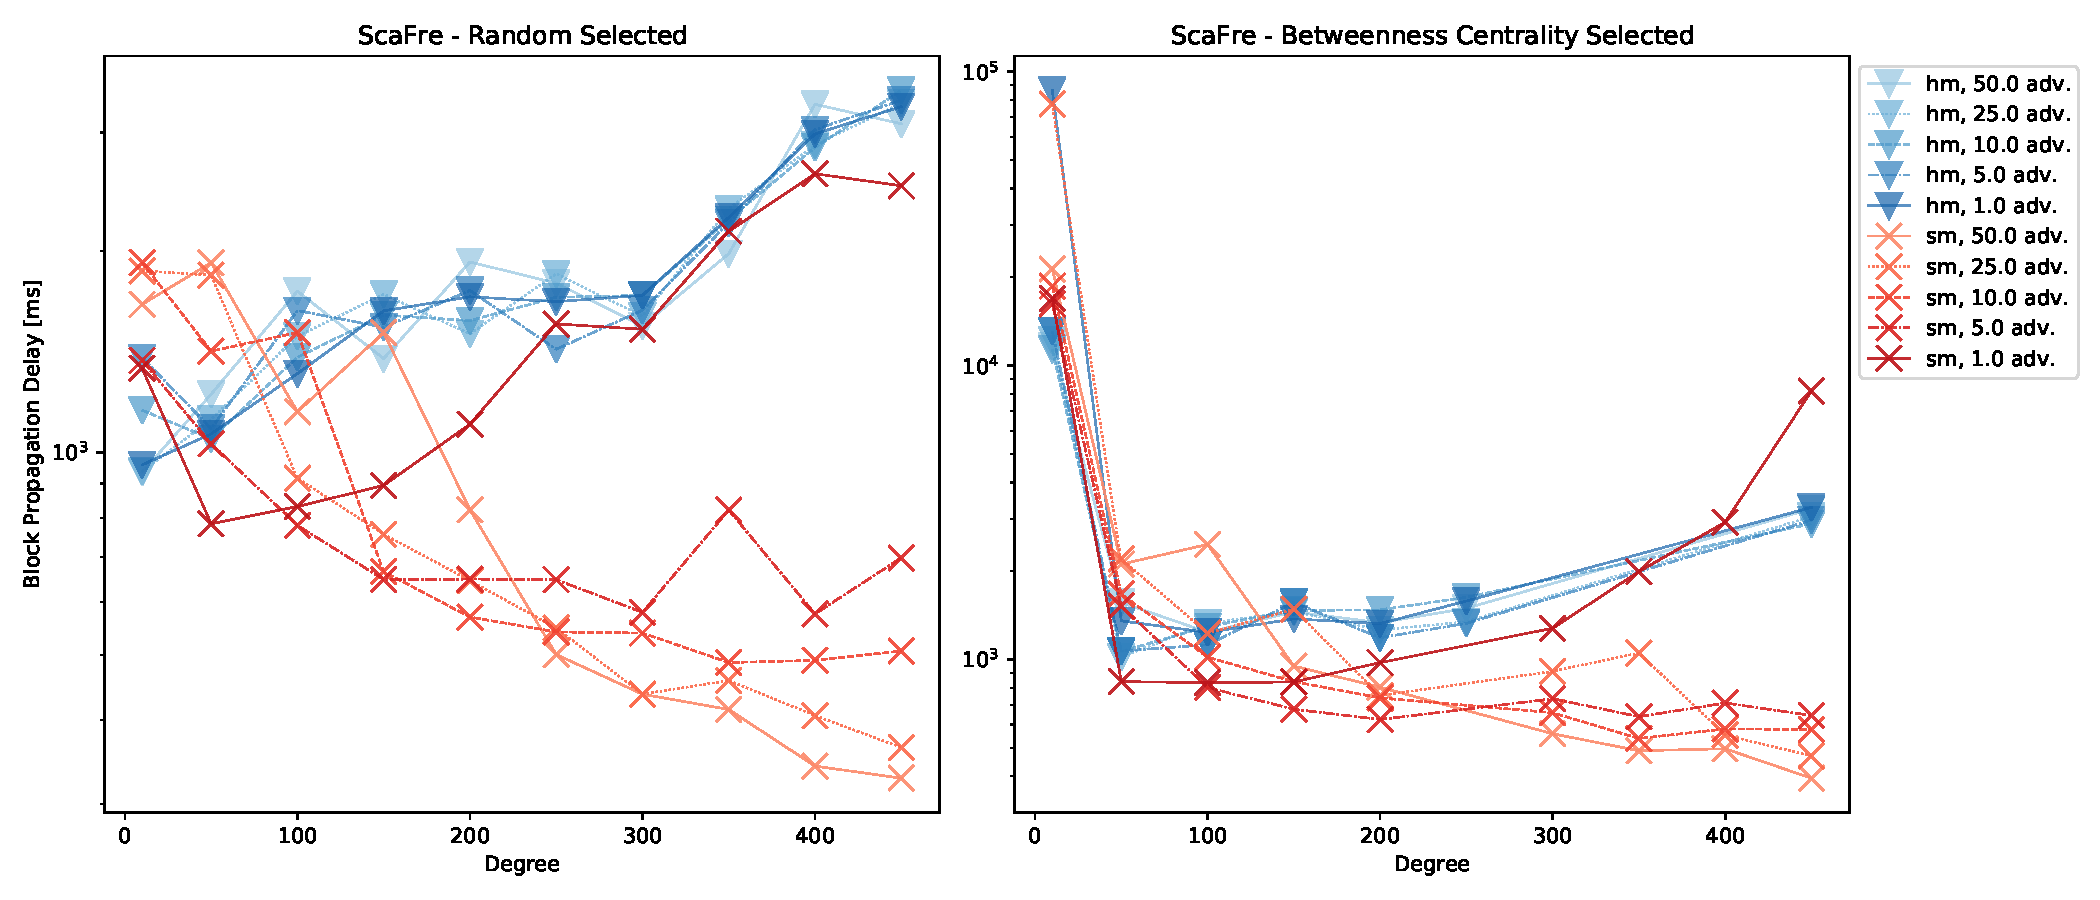
\includegraphics[width=\textwidth]{figures/sm_edge_block_scafre.pdf}
		\caption{$ScaFre$ simulation setup}
		\label{fig:blockprop_bara}
	\end{subfigure}
	\begin{subfigure}[b]{\textwidth}
		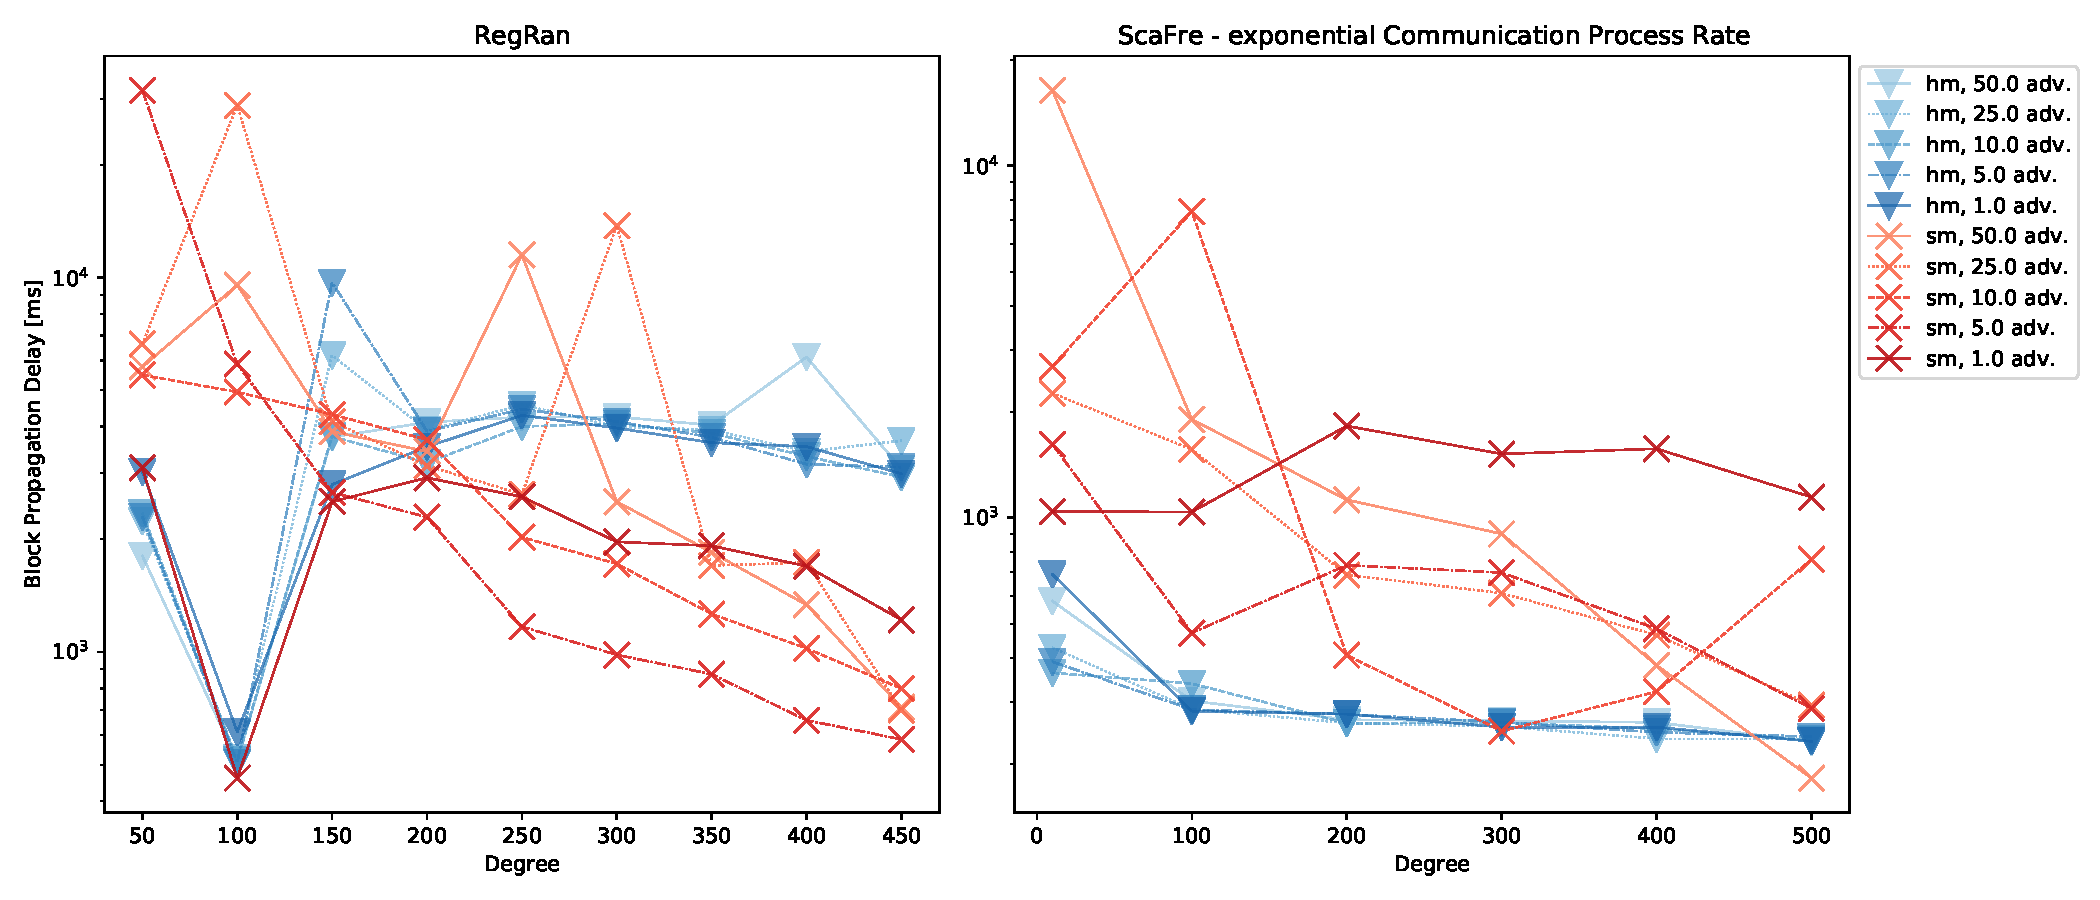
\includegraphics[width=\textwidth]{figures/sm_edge_block_prop_rr_and_bc_dc.pdf}
		\caption{$RegRan$ and $ScaFre$- exponential distributed communication process rate simulation setup}
		\label{fig:blockprop_2}
	\end{subfigure}
\caption{Block Propagation delay of Blocks mined by peer with ID $0$}
\label{fig:blockprops}
\end{figure}\\
Figure\ref{fig:blockprop_bara} shows the  block propagation delay of blocks mined by peer with ID $0$ for the $ScaFre$ simulation setup. Especially for honest mining we can see an increasing block propagation delay for an increasing degree. Since blocks of peer with ID $0$ need more time to propagate through the network it is less likely that those blocks will be part of the main chain. This results in a revenue loss. For selfish mining we observe a similar behavior. Selfish mining with no communication process rate advantage shows the least amount of revenue gain. We also observe a very high block propagation delay for 10-degree in the betweenness centrality selected simulations. We deduce that high centrality peers in this setup are a bottleneck. In the $ScaFre$ setup every peer has the same average communication process rate. This results in a higher average time to cover all edges for a peer with a higher degree. Thus, this peer becomes a bottleneck and it is not beneficial to connect to those peers with the highest centrality. This also explains why it is beneficial for the selfish miner to have a higher degree once he has a communication process rate advantage, since then he can effectively use multiple parallel paths to propagate his blocks faster. We also see this behavior in Figure~\ref{fig:blockprops} since for communication process rate advantages and higher degrees the selfish miner achieves lower block propagation delays.\\
For the $RegRan$ block propagation delays we observe a more diverse picture. For an increased degree and communication process rate advantage we observe lower block propagation times for the selfish miner. For the honest miner we observe the minimal block propagation at 100-degrees. The overall block propagation delay is higher than in the $ScaFre$ experiments for the honest miner, which would explain the reduced revenue gain. This leads to the assumption that for honest mining a lower block propagation delay is correlated to a higher revenue gain.\\
Figure~\ref{fig:blockprop_2} visualizes the block propagation delay for a modified $ScaFre$ setup. In $ScaFre$ node degrees are exponentially distributed, but the communication process rate is constant. To further evaluate if central nodes become bottlenecks the modified $ScaFre$ setup scales communication process rate distribution to degree distribution. A high degree node with the same communication process rate as a low degree node needs more time to cover all of his connections. The modified $ScaFre$ setup scales communication process rates in such a way, that the average round trip time remains the same, independent of node degree.
\begin{figure}[tbp]
	\begin{subfigure}[b]{\textwidth}
		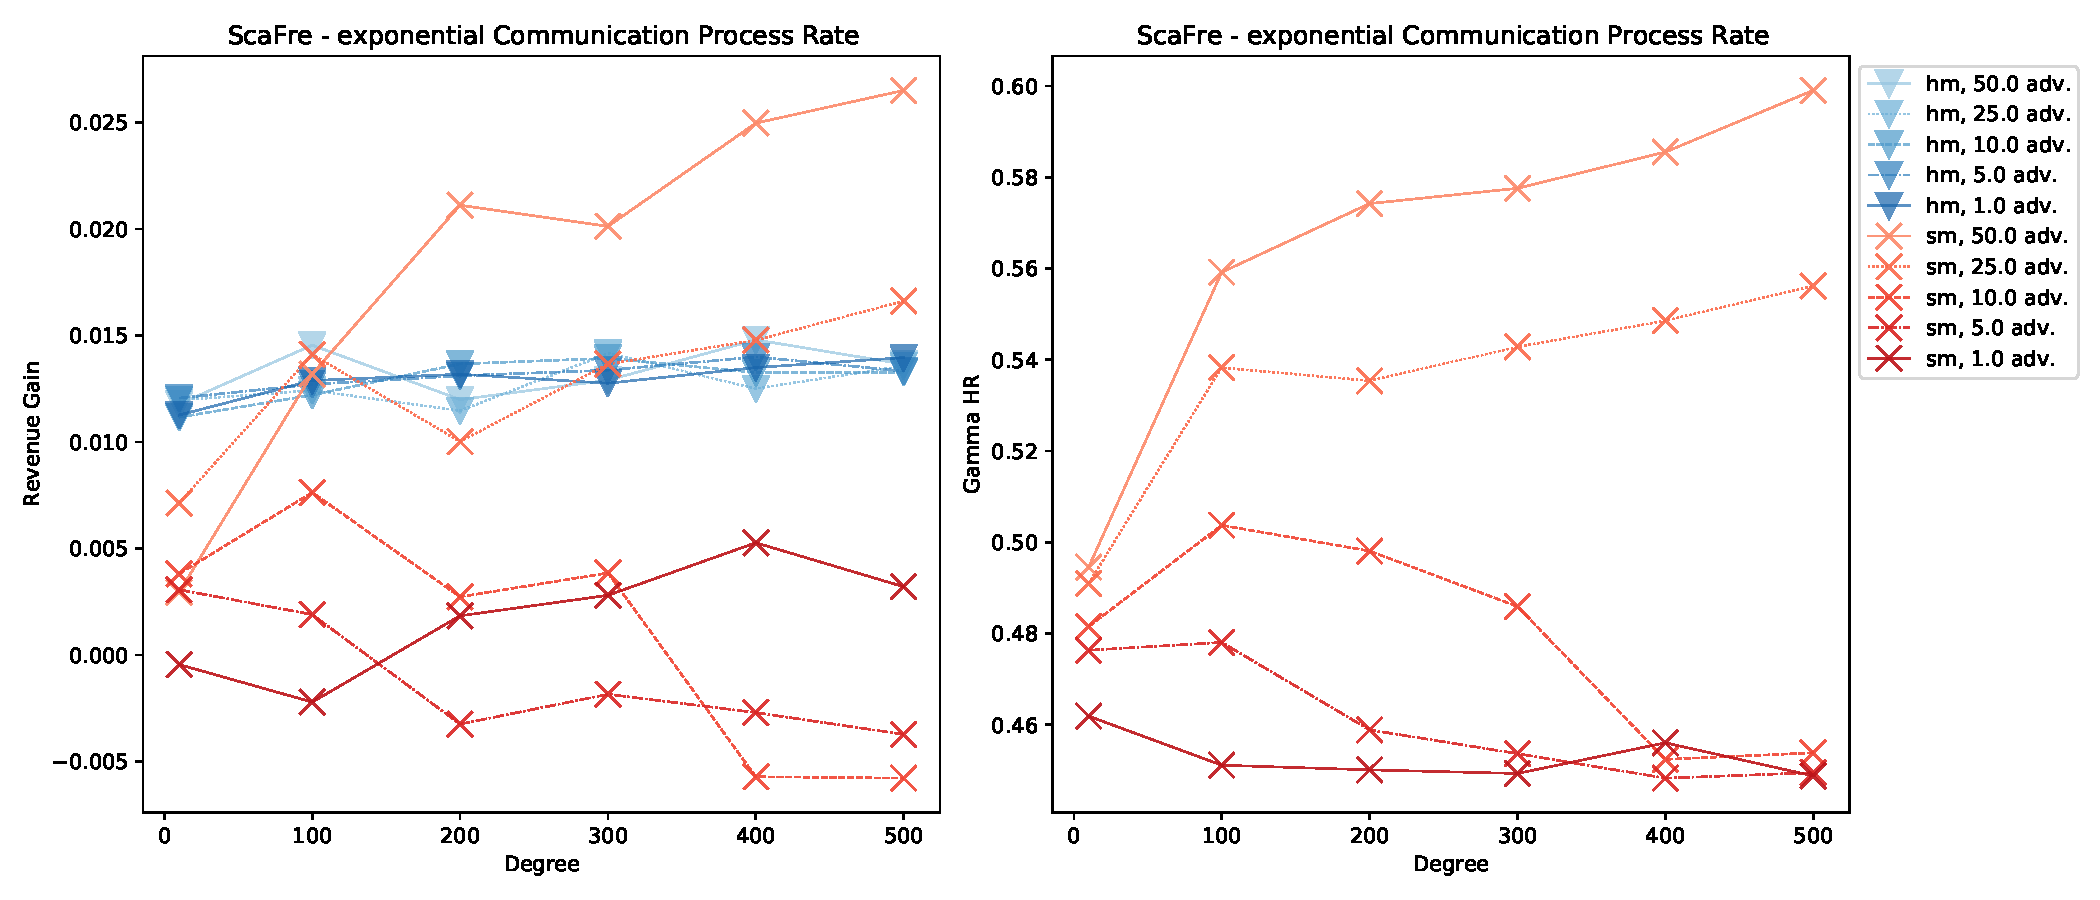
\includegraphics[width=\textwidth]{figures/revenue_gamma_barabasi_bc_dc.pdf}
		\caption{Revenue Gain and Gamma}
		\label{fig:revgain_bc_dc}
	\end{subfigure}
	\begin{subfigure}[b]{\textwidth}
		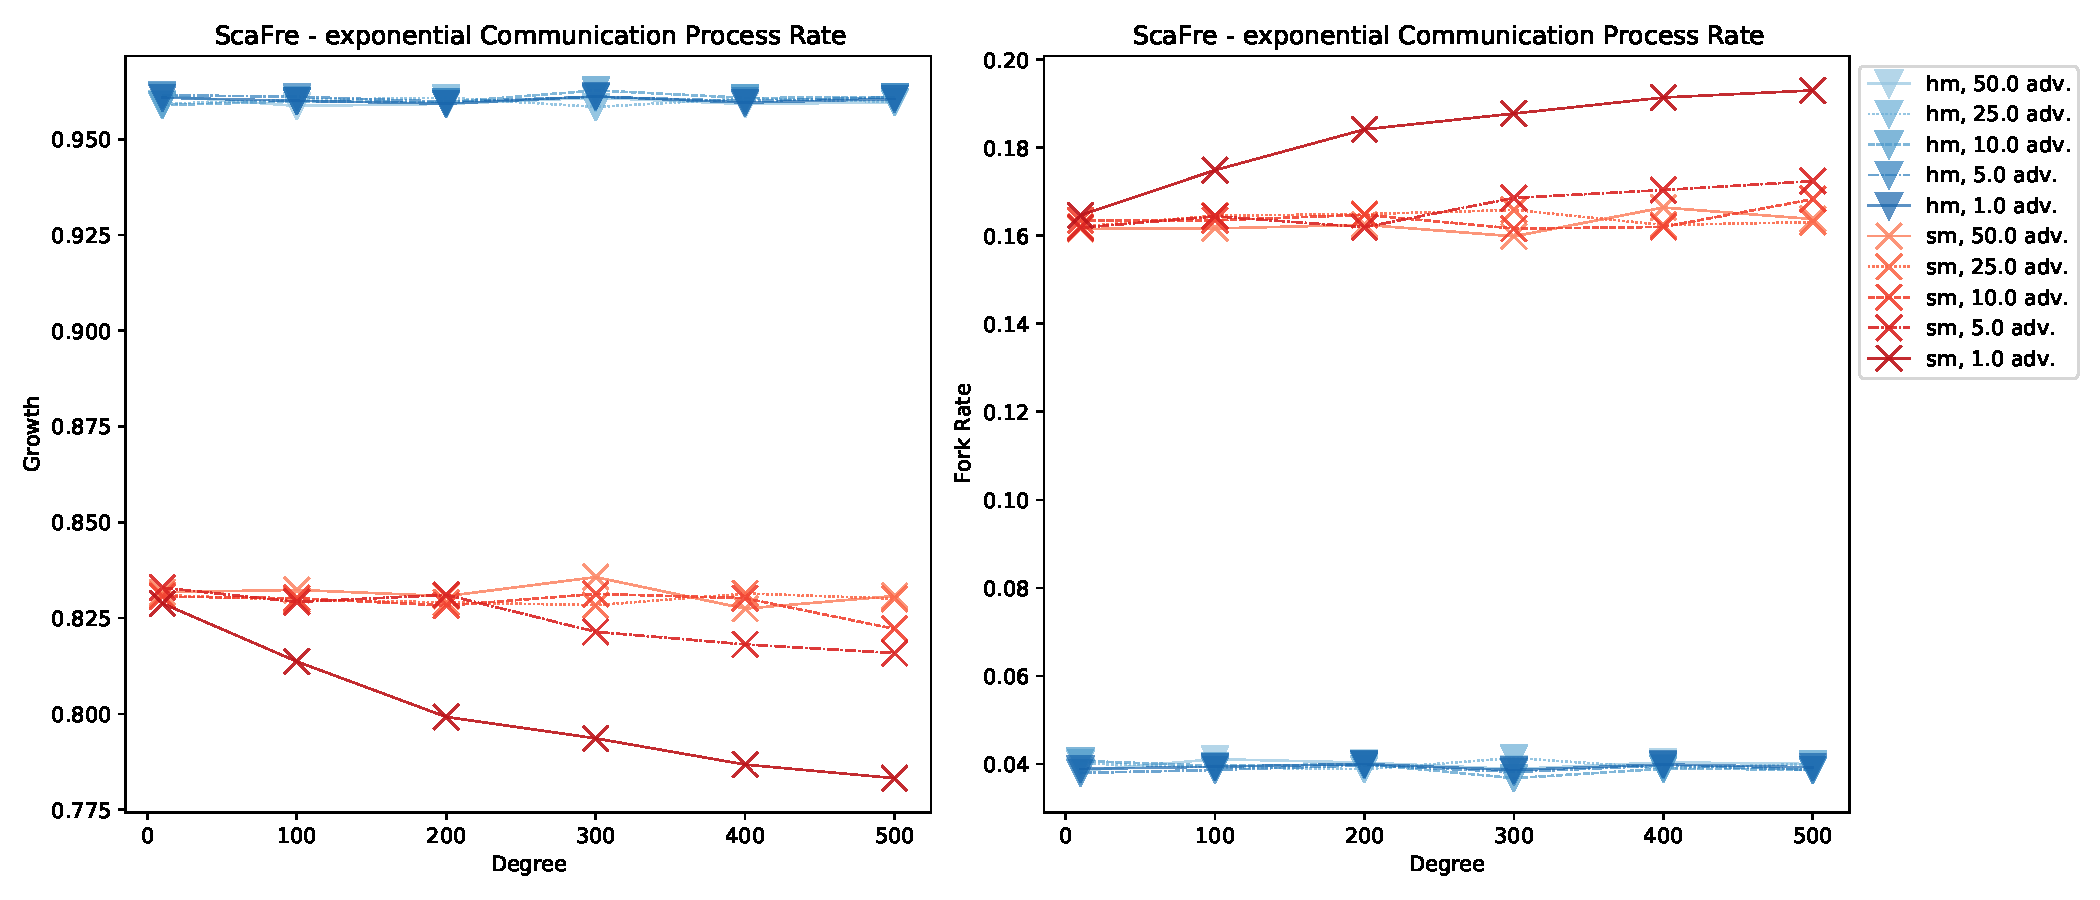
\includegraphics[width=\textwidth]{figures/growth_forkrate_barabasi_bc_dc.pdf}
		\caption{Growth and Fork Rate}
		\label{fig:growth_bc_dc}
	\end{subfigure}
\caption{Simulations $ScaFre$ with exponential Communication Rate Distribution Setup with Network Advantage for honest mining(hm) and selfish mining(sm), Different Communication Process Rates Advantages}
\label{fig:bc_dc}
\end{figure}\\
Figure~\ref{fig:blockprop_2} shows the block propagation delay for peer with ID $0$ in this modified topology. We observe that the honest miner can transmit his blocks faster. Overall the system seems more stable since $growth$ is higher than in $RegRan$ and $ScaFre$ and the $fork~rate$ is lower. This is visualized in \ref{fig:growth_bc_dc}. Figure~\ref{fig:revgain_bc_dc} visualizes $revenue~gain$ and $\gamma_{HR}$. The honest miner has a lower and constant $revenue~gain$ compared to previous experiments. This in conjunction with the higher $growth$ implies that the network is more stable in this modified version. The selfish miner experiences a lowered $revenue~gain$ as well. However, we do not observe lower values of $\gamma_{HR}$. The reduced $revenue~gain$ must therefore be a result of the increased $growth$ and reduced $fork~rate$. This seems intuitive because as stated by \cauth{eyal} selfish mining benefits from an increased number of forks.\\
To sum up we observe major key relations between different system parameters. Selfish mining does in fact produce an increased revenue if network advantage and relative hashrate exceed a certain threshold. In fact we observe a revenue gain up to $0.052$ for a high network advantage. For a relative hashrate of $45\% $ we observe the needed network advantage to consist of an increased bandwidth by a factor 5 to 25 and the ability to establish more connections. The actual threshold highly depends on the topology and overall characteristic of the rest of the network. We observe that selfish mining is more effective in a system with a reduced growth of the blockchain. Additionally a relationship of $growth \approx 1-fork~rate$ is clearly visible, which implies that forks mainly consist of 1 block. Honest mining produces an increased revenue as well. For the tested high relative hashrate of $45\% $ honest mining produced a revenue gain between $0.01$ and $0.045$. Additionally we see that the produced revenue of honest mining highly depends on the performance of the rest of the network. This is in contrast to selfish mining. While selfish mining also depends on the rest of the network, revenue can increase by increasing bandwidth and degree of the selfish miner. Overall we see a high dependence between the performance of selfish mining and network advantage of the peer executing the attack.\\
From a more general point of view we see that revenue does not solely depend on relative hashrate. It is a combination of relative hashrate, selected mining strategy and network characteristics. The selected mining strategy is influenced by different network effects. Honest mining is strongly influenced by the overall network and can produce revenue gain. Selfish mining is strongly influenced by the network advantage a peer possesses. Without a high hashrate and network advantage selfish mining is outperformed by honest mining. However, we observe that selfish mining can outperform honest mining with a high enough relative hashrate and network advantage.









 
